\chapter{Implementation}
This chapter is concerned with the implementation details of the individual components introduced in Chapter \ref{chapter:4}. This includes the development of the Unity application responsible for producing the front-facing camera video stream and displaying the visual cues, the development of the human detection and direction system, as well as the reactive control systems implemented for the control of ARTA. Previous work in the PRL had utilized the Hololens camera to capture images that were then processed on an external computer, but where this project differs is that a video stream is required to perform real-time object detection. As such, a large amount of time was spent at the very beginning of the project trying to produce a video stream, since the whole project depended on this form of visual input.

\begin{figure}[ht]
    \centering
    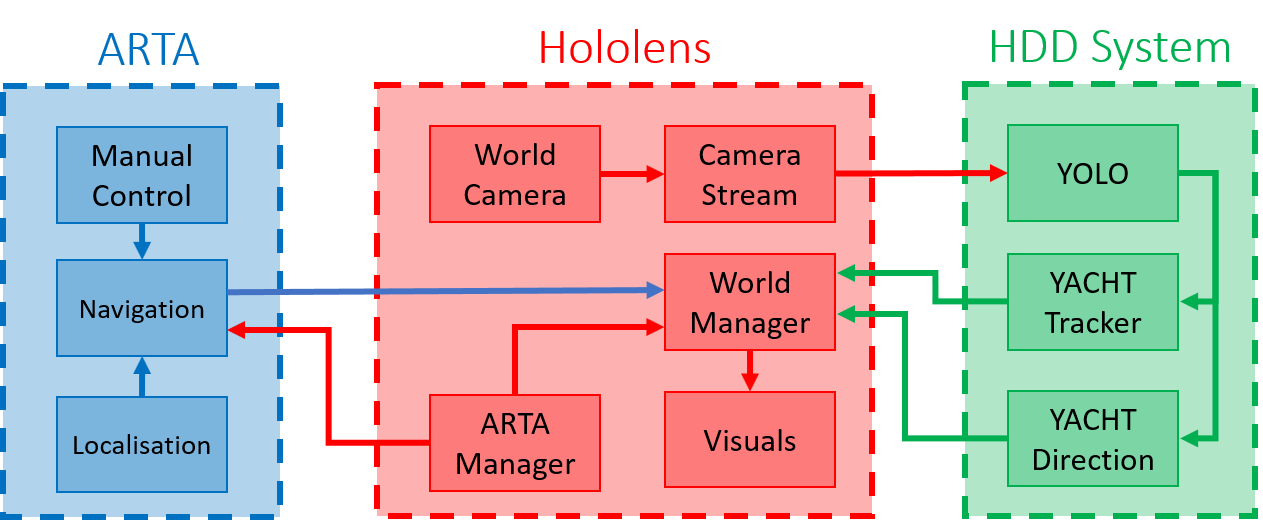
\includegraphics[width=1.0\linewidth]{img/chapter5_implementation/detailedSystemDiagram.png}
    \caption{System diagram detailing individual components of the programs running on each device.}
    \label{fig:detailedHL}
\end{figure}

Figure \ref{fig:detailedHL} is a more detailed diagram of the high level system digram presented in Figure \ref{fig:simplifiedHL}. We show the communication between the three separate devices, and how each node can be broken down into smaller nodes running specific computations. For the rest of this report, we represent the ARTA, Hololens, and HDD system components with the colours blue, red, and green respectively.

\section{Human Detection \& Direction System}
In order to determine the direction people are walking in, it is necessary for the system to be able to detect humans. Only after detection is it possible to discern the motion of individuals, which can be achieved through object tracking and body pose estimation. Figure \ref{fig:detailedHDD} shows the breakdown of the HDD node into components responsible for these two tasks. This section is concerned with the implementation of the methods needed to perform the direction prediction, as well as how the system communicates between its nodes. 

\begin{figure}[ht]
    \centering
    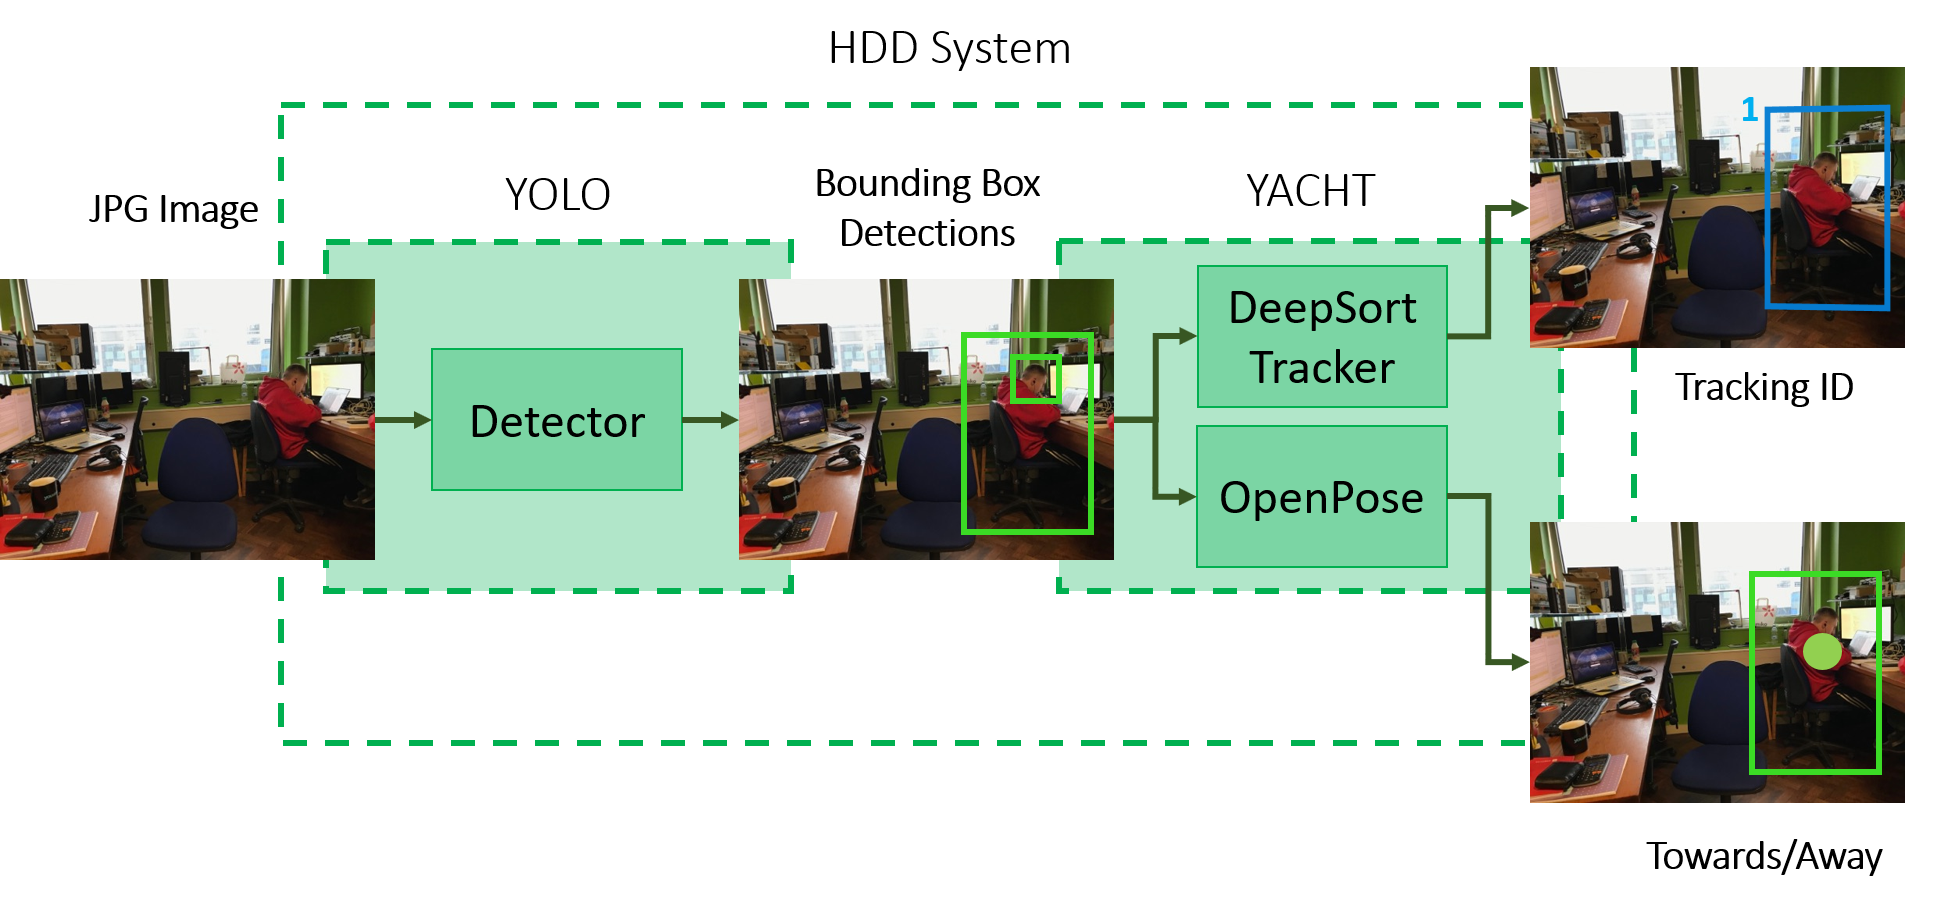
\includegraphics[width=1.0\linewidth]{img/chapter5_implementation/hddSystemDiagram.png}
    \caption{The HDD System is sub-divided into two ROS packages, YOLO and YACHT. We show that YACHT has two sub-nodes which both depend on the outputs of the detector.}
    \label{fig:detailedHDD}
\end{figure}

We begin this section by listing the hardware requirements for the system. Due to the nature of the HDD, and its reliance on modern deep learning techniques, access to a modern GPU is essential. We refrain from trying to explain the step-by-step process to setup the hardware and software, and instead, point the reader in the direction of an article\footnote{https://link.medium.com/xQ5w2FMXoX} which covers this topic.

\subsection{Hardware \& Software Dependencies}

\subsubsection{Hardware}
We implemented the HDD system on a desktop computer connected to the Imperial College network. Due to the real-time computer vision requirements of this project, the computer was chosen due to the GTX 1050Ti GPU with 4GB video RAM available on the system. The computer was also equipped with an Intel i7-2600 CPU and 8GB DDR3 RAM.

\subsubsection{Software}
We have refrained from posting all Python dependencies for the project and only mention the important ones. A complete listing is available in the corresponding repositories of the packages. The following software dependencies are required to run this project:
\begin{itemize}
    \item Ubuntu 16.04
    \item Python 2.7
    \item OpenCV 3.0
    \item ROS Kinetic
\end{itemize}

Due to the deep learning component of the project, the following software dependencies are essential:
\begin{itemize}
    \item Nvidia Graphics Drivers 
    \item CUDA 8.0 Toolkit
    \item cuDNN 6.0
    \item Darknet
    \item Tensorflow-GPU
    \item Caffe
\end{itemize}

\subsection{YOLO Object Detector}
As mentioned in Section \ref{sec:yolo}, we chose to use the YOLOv3 Tiny architecture and trained it on the CrowdHuman dataset. We begin this section by introducing the reader to \textbf{Darknet}, the neural network framework YOLO is implemented on, and how we integrated it into ROS. We also briefly explain how the network detects objects and compare YOLOv3 Tiny with the more memory intensive YOLOv3. We then guide the reader through the training process, and the analysis we did to validate the human detection improvements compared to pre-trained models.

\subsubsection{Darknet}
Darknet\footnote{https://pjreddie.com/darknet/} is an open source neural network framework written in C and CUDA which supports both CPU and GPU computation \cite{darknet13}. The source code for the framework is freely available on GitHub, and it can be used to train different neural network architectures like more conventional deep learning frameworks such as Tensorflow or Caffe.

\subsubsection{Darknet in ROS}
By definition, ROS is language-independent, although, at the time of writing, three main libraries have been defined for ROS, making it possible to program ROS in Python, Lisp or C++. On the other hand, Darknet is implemented in C, due to the speed of compiled low-level languages in conjunction with CUDA. However, the Darknet framework is compiled into \textit{Shared Object (.so)} file, which is analogous to a Windows DLL. As such, it becomes possible to access the framework by writing wrappers around the compiled library file.

\paragraph{}Darknet has basic Python wrappers around the compiled library which convert Python data types into C and vice versa. However, the original wrappers for detection are written to run on images that are saved on disk. Darknet converts the saved images into a C data structure \code{IMAGE} and performs the detections. To integrate the framework into ROS, the node must be able to receive data from image topics with \code{CompressedImage} or raw \code{Image} messages.

\paragraph{}In ROS Python, the JPG or PNG images received from the \code{CompressedImage} message can be converted to numpy arrays which store the RGB values, without the need to be saved on disk. As such, we wrote Python wrappers for Darknet that allow the framework to support images in the form of numpy arrays as well as images saved on disk. The following listing defines the \code{IMAGE} data structure, and the conversion of an image numpy array to the Darknet format: \\

\begin{lstlisting}[language=Python, caption={Darknet IMAGE Python wrappers for seamless ROS integration.}]
# IMAGE: a C data structure used by Darknet
class IMAGE(Structure): 
    _fields_ = [("w", c_int),
                ("h", c_int),
                ("c", c_int),
                ("data", POINTER(c_float))]
                
# Converts numpy array to Darknet IMAGE type
def nparray_to_image(img): 
    data = img.ctypes.data_as(POINTER(c_ubyte))
    image = ndarray_image(data, img.ctypes.shape, img.ctypes.strides)

    return image
\end{lstlisting}

Further Python wrappers were written for the detection and return of the image bounding box co-ordinates. We also created ROS messages for the bounding box detections, which allows the Darknet YOLO node to communicate with other nodes in the HDD system. The full code listing can be found in the Appendix \footnote{https://github.com/alaksana96/darknet-crowdhuman}\footnote{https://github.com/alaksana96/fyp\_yolo}.

\subsubsection{YOLO Detection Algorithm}
As researched in Section \ref{sec:backYOLO}, the algorithm divides an input image into a $S\times S$ grid. Each grid cell can predict one object, and a cell can predict a fixed number of bounding boxes $B$, which we visualize in Figure \ref{fig:yoloViz}. The predicted bounding box is chosen from the set of $B$ boxes with the highest box confidence score, which is a measure of how likely the box contains an object and how accurate the boundary box is. It also predicts the conditional class probability, which is the probability a detected object belongs to a particular class. 

\begin{figure}[ht]
    \begin{subfigure}[b]{.45\textwidth}
        \centering
        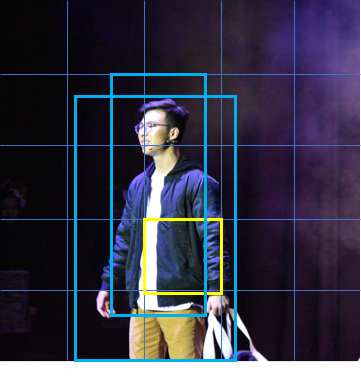
\includegraphics[width=1.0\linewidth]{img/chapter5_implementation/yoloAlgo1.png}
        \caption{A grid cell can make $B$ predictions, in this example $B=2$.}
    \end{subfigure}%
    \hspace{\fill} 
    \begin{subfigure}[b]{.45\textwidth}
        \centering
        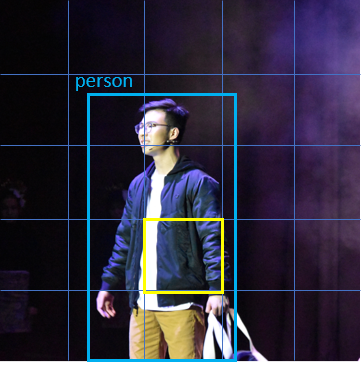
\includegraphics[width=1.0\linewidth]{img/chapter5_implementation/yoloAlgo.png}
        \caption{The bounding box with higher box confidence score is used.}
    \end{subfigure}
    \vspace{-1\baselineskip}
    \begin{center}
        \caption{Visualization of the YOLO person detection algorithm dividing a resized square image into grid cells.}
        \label{fig:yoloViz}
    \end{center}
    \vspace{-2\baselineskip}
\end{figure}

\subsubsection{YOLOv3 Tiny vs YOLOv3}
While testing out the different models, we noticed that the YOLOv3 model was consistently crashing and causing segmentation faults. On further investigation, we noticed that this was due to the network using up all 4GB of video memory available on the GPU. In comparison to its predecessors YOLO and YOLOv2, YOLOv3 is a much larger network which has 106 fully convolutional layers. Although it is far more accurate at predicting bounding boxes, it reduces the frame rates that can be achieved on video. As such, we decided to use YOLOv3 Tiny, a shallower variant of the network that is suitable for real-time image detection. Although the tiny version is not as accurate, it is much lighter on memory, using less than 1GB video RAM, making it a suitable choice for this project.

\subsubsection{Training YOLOv3 Tiny}
\paragraph{CrowdHuman} The CrowdHuman dataset \cite{Shao} is a benchmark dataset to evaluate detectors in crowd scenarios better. The essential features of the dataset are the size, quality of the annotations, and diversity. Each image contains multiple people with varying degrees of occlusion, which allows for object detectors to better learn the representation of obscured people. 

\begin{figure}[ht]
    \centering
    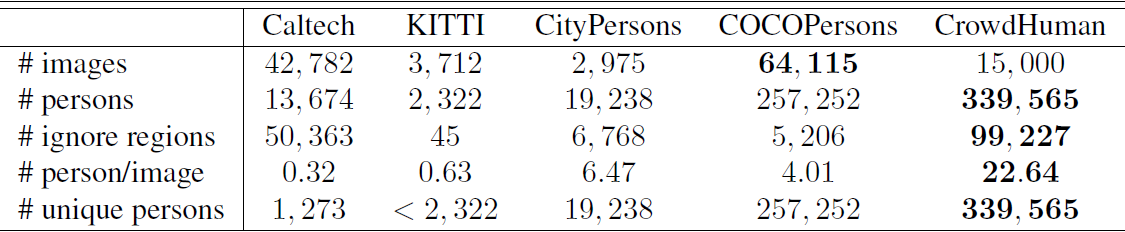
\includegraphics[width=0.9\linewidth]{img/chapter5_implementation/crowdHumanStats.png}
    \caption{A comparison of CrowdHuman to other person image datasets \cite{Shao}, showing the increase in number of people and diversity in the images.}
    \label{fig:crowdHumanStats}
\end{figure}

As can be seen from Figure \ref{fig:crowdHumanStats}, the dataset contains far more unique identities. By examining the dataset, we can see that it contains people in a wide array of situations, at varying distances with different body poses.

\paragraph{Annotations} The CrowdHuman dataset provides its annotations in the \code{.odtg} format, which is a variant of JSON. Each line in the annotation file corresponds to a JSON containing the image ID and the bounding boxes. The annotations include boxes for the \textit{visible box}, \textit{full body box} and \textit{head box}. For training, we chose to use the full body and head boxes only. We wanted the detector to be able to learn to predict occluded individuals, and we also wanted to experiment with head pose estimation. Each bounding box is annotated as below, where \code{x,y} is the top-left corner of the bounding box. The \code{width} and \code{height} are also given in image co-ordinate pixels.

\paragraph{}\code{[x, y, width, height]}  

\paragraph{}On the other hand, to train YOLO on Darknet, the annotations must be given in a completely different format. The Darknet annotation format is as such:

\paragraph{}\code{<object-class> <x> <y> <width> <height>}

\paragraph{}Since Darknet accepts images of any size; it works with image units which are scaled relative to the size of the image. As such, all the values for the bounding boxes are between $0$ and $1$. Furthermore, the \code{x, y} values in the annotation are measured from the centre of the bounding box.  

\paragraph{Converting Annotations} To use the CrowdHuman images as a training set for the YOLOv3-tiny model, we had to write several scripts that converted the annotations to the Darknet format. We have included these scripts in the Appendix should the reader wish to convert the dataset themselves\footnote{https://github.com/alaksana96/darknet-crowdhuman/blob/master/README.md}.

\paragraph{Training Parameters} Before training, we set up the model configuration file to learn two classes, head, and body, as well as to use batches of 32 divided into a subdivision of 8 images. This limits the number of images loaded into memory at once to 8, to prevent running out of GPU memory. We also reduce the size of the training images to $416\times 416$ pixels, to further reduce the GPU usage. \\

\begin{lstlisting}[language=Mymatlab,caption={Training parameters used for YOLOv3 Tiny on the CrowdHuman dataset}]
    batch=32 %Training parameters for YOLO Tiny
    subdivisions=8
    width=416
    height=416
    channels=3
    momentum=0.9
    decay=0.0005
\end{lstlisting}

These optimizations were done to maximize the amount of GPU memory used for training, without a sudden surge in usage causing a segmentation fault. Resizing the input training images allows the algorithm to divide the image into a $S\times S$ grid. Generally, the larger the height and width, the better the predictions, since the image can be divided into more grid cells. This is a trade-off we had to make to be able to train the network on a mid-range GPU.

\paragraph{Training Process} We left the model to train overnight, creating backups of the weights every 1000 iterations. The following day, after reaching 30,000 iterations, we decided to stop training the network. The average loss error and total loss had stopped decreasing for several hours and was hovering at around $29.134$. We reasoned that the network had reached a minimum, and further training would be redundant since it would over-fit the dataset. The final weights are available in the file \code{yolov3-tiny-crowdhuman.backup}.

\subsubsection{Evaluating Trained Model}
\paragraph{Hololens Videos} As mentioned in Section \ref{sec:backYOLO}, we recorded several test videos using the Microsoft Hololens. These videos were capture in various locations on the Imperial College campus. Figure \ref{fig:yoloRange} shows the model detecting people at range.  

\begin{figure}[ht]
    \centering
    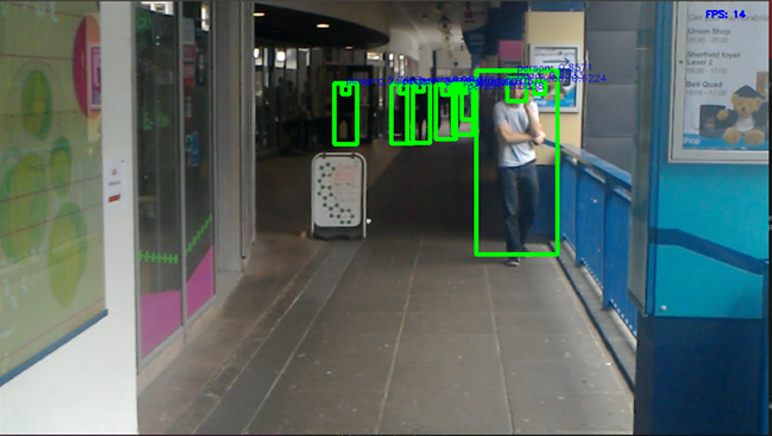
\includegraphics[width=0.5\linewidth]{img/chapter5_implementation/yoloWalkway.png}
    \caption{Trained model detects people and heads at different ranges. We also see it can detect people far away and accurately detect their heads.}
    \label{fig:yoloRange}
\end{figure}

A common area where lots of people frequent is Sherfield walkway. As seen in Figure \ref{fig:yoloSherfield}, this was an ideal place to capture a video since it features a lot of people walking around in different directions. We obtained several more videos outside the EEE building and inside the 5th floor ICRS lab.

\begin{figure}[ht]
    \centering
    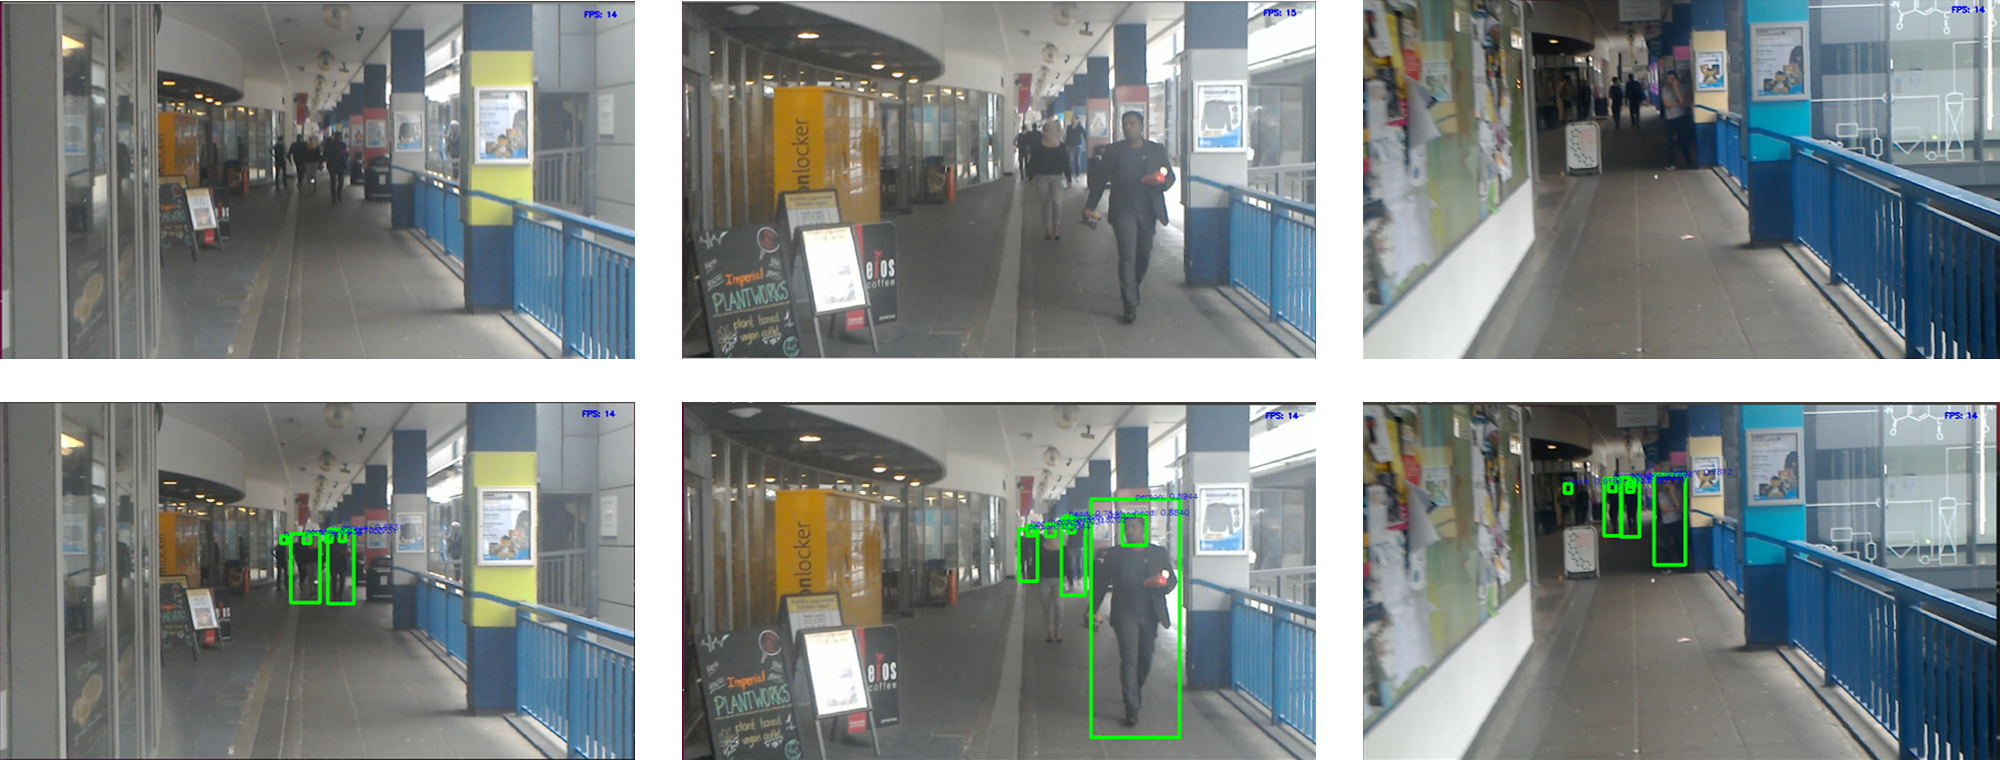
\includegraphics[width=0.95\linewidth]{img/chapter5_implementation/yoloWalkwayMultiple.png}
    \caption{Evaluating the model on Sherfield Walkway test video. We notice that it is able to small figures close together at a distance.}
    \label{fig:yoloSherfield}
\end{figure}

The videos from the Hololens were captured whilst a person was walking with the device, to best emulate a PWU in a wheelchair navigating through populated areas. We noticed an improvement in the number and accuracy of the detected bounding boxes compared with the pre-trained COCO models provided by Darknet. 

\subsubsection{ROS Node} \label{sec:nodeYOLO}
The Python wrappers for Darknet allow us to access the detection and image conversion functionality of the framework. To fully integrate the framework as a ROS node, we must follow the standard ROS procedures for creating a new ROS package. As such, we have created a package\footnote{https://github.com/alaksana96/fyp\_yolo} that runs Darknet and YOLO that can be downloaded and run seamlessly with ROS.

\paragraph{ROS Topics} The ROS node subscribes to the \code{/image\_transport/compressed} and expects to receive images in the compressed JPG format. This is because the Hololens captures video frames and encodes it to reduce the usage on the network bandwidth. These images are converted to numpy arrays which are then converted to Darknet \code{IMAGE} types for detection. 

\paragraph{} Darknet produces bounding box co-ordinates and class probabilities for each detection in an image. For every received frame, the node publishes the original image and a list of associated bounding boxes. The bounding box message contains the following information: \\

\begin{lstlisting}[language=Mymatlab,caption={BoundingBox.msg},label={bbmsg}]
string Class
float64 probability
int64 xmin % Top Left Corner
int64 ymin
int64 xmax % Bottom Right Corner
int64 ymax
\end{lstlisting}

\subsection{YACHT Package} \label{sec:YACHT}
The major contribution of this project is in the form of the Yet Another Crowd Human Tracker package for ROS. This package utilizes the Deep SORT algorithm and OpenPose body pose estimation framework to determine the direction of individuals.

\paragraph{ROS Communication} As seen in Section \ref{sec:nodeYOLO}, the YOLO object detector node publishes a topic which contains the image and associated bounding boxes. Figure \ref{fig:detailedHL} shows that both YACHT nodes subscribe to the same output topic. The reason we decided to include the original image in the message and not just the bounding boxes is so that we can be sure the bounding boxes were detected for that frame, without having to subscribe to two separate topics and comparing timestamps on individual messages.

\subsection{YACHT: Tracker}
As explained in Section \ref{sec:YACHT}, the YACHT tracker depends on the Deep SORT algorithm \cite{Wojke2018}. Using the detections produced by the YOLO node, we assign IDs and match them across video frames to produce a track. These tracking IDs are then sent to the Hololens for visualization.


\subsubsection{Deep SORT} 

\paragraph{Modifications} We have modified\footnote{https://github.com/alaksana96/deep\_sort} Nicolai Wojke's original implementation of Deep SORT to run on Tensorflow-GPU. In the original, as the number of detections increased, so does the delay in tracking. This issue is more prevalent when tested on the MOT dataset, which has a large number of objects in each frame. Figure \ref{fig:deepSortCPU} visualizes the delay on the MOT16-06 video. We can see that the algorithm is operating at a very low FPS, causing it to be delayed in time. 

\begin{figure}[ht]
    \begin{subfigure}[b]{.45\textwidth}
        \centering
        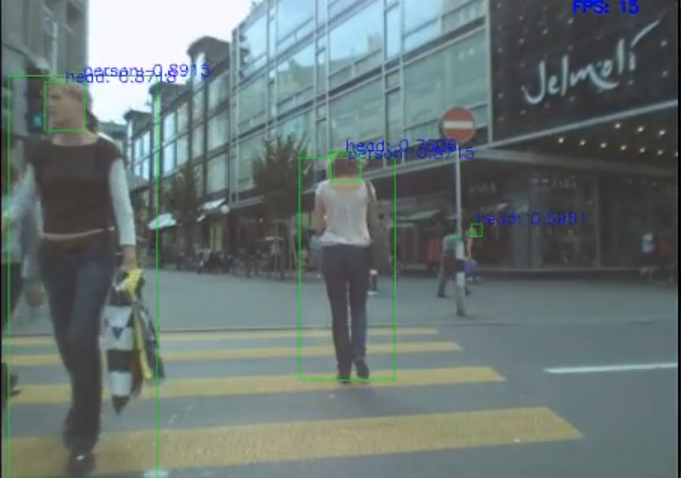
\includegraphics[width=1.0\linewidth]{img/chapter5_implementation/deepSortCPU.png}
        \caption{Output of YOLO. The image frame and bounding boxes are fed to Deep SORT}
    \end{subfigure}%
    \hspace{\fill} 
    \begin{subfigure}[b]{.45\textwidth}
        \centering
        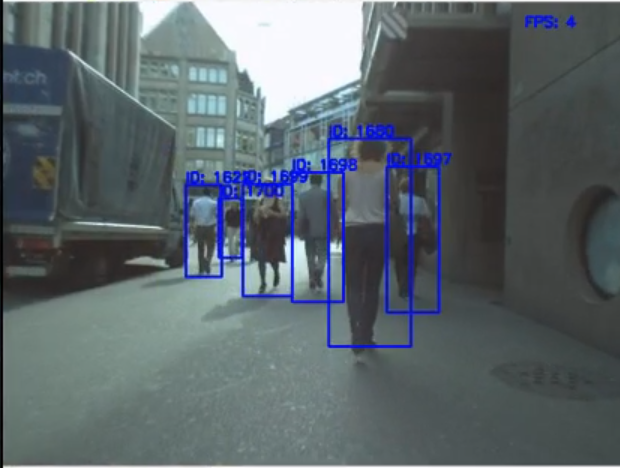
\includegraphics[width=0.935\linewidth]{img/chapter5_implementation/deepSortCPU1.png}
        \caption{Deep SORT is several frames behind since it runs at 4 FPS}
    \end{subfigure}
    \vspace{-1\baselineskip}
    \begin{center}
        \caption{Visualization of delay on CPU bound Deep SORT}
        \label{fig:deepSortCPU}
    \end{center}
\end{figure}


\paragraph{Deep Association Metric} Through code profiling, we noticed that the program was spending a lot of time in the generation of feature vectors. Upon inspection, we noticed that this process was run on a CPU bound version of Tensorflow. The \code{ImageEncoder} class uses a pre-trained deep network that generates the feature vectors for each bounding box. By using Tensorflow-gpu, we were able to run the network on the system GPU, removing the delay. \\

\begin{lstlisting}[language=Python, caption={Deep SORT Tensorflow GPU modifications}]
class ImageEncoder(object):

    def __init__(self, checkpoint_filename, input_name="images",
                 output_name="features"):
                 
        # Tensorflow-GPU
        gpu_options = tf.GPUOptions(per_process_gpu_memory_fraction = 0.2)
        self.session = tf.Session(config=tf.ConfigProto(gpu_options=gpu_options))
\end{lstlisting}

\paragraph{Trackers \& Tracking} For each detection, we generate a feature vector using the image pixels within the bounding box. A matching cascade with Nearest Neighbour metric is used to best match the detection with existing confirmed tracks. Some detections will not get matched since the distance to confirmed tracks is above the \code{matching\_threshold}. The algorithm then attempts to match the detections to unconfirmed tracks using a simple Intersection-over-Union metric. These are newly created tracks that have existed for less than the last $n$ frames. If the detection is still unmatched, the algorithm creates a new tracker for the detection and adds it to the pool of unconfirmed tracks.

\begin{figure}[ht]
    \centering
    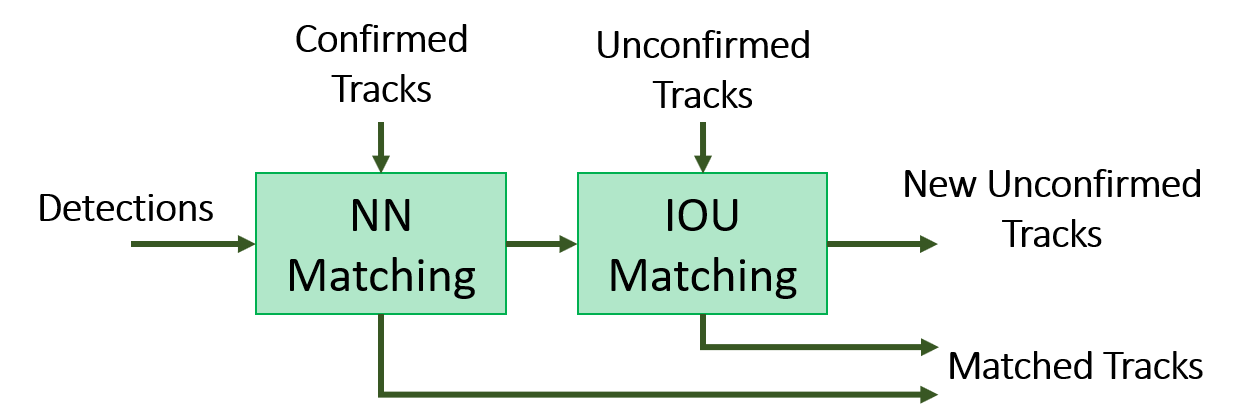
\includegraphics[width=0.8\linewidth]{img/chapter5_implementation/deepSortMatching.png}
    \caption{Visualization of Deep SORT matching. IOU matching is used as a final check for tracks that are unmatched by feature vector Nearest Neighbour matching.}
    \label{fig:deepSortMatch}
\end{figure}

Any pre-existing tracks which are not matched are checked. If the number of frames since the previous match is greater than the \code{max\_age} parameter, the track is considered dead and is deleted. This is done to prevent the number of tracks from growing infinitely. A Kalman filter is used to update the bounding box states of each track, as well as the time since the last update.
 
\subsubsection{Linear Extrapolation}
We experimented with linear extrapolation across frames as a way of inferring the direction travelled by the detection. As the project progressed, we encountered issues with this method, as explained in Section \ref{sec:objecTrackingDirection}. By searching for alternative methods, it was found that the depth camera on the Hololens can determine the distance between the PWU and an object relatively accurately. As such, we abandoned the pure computer vision approach in favour of using the Hololens.

\subsubsection{ROS Topic} \label{sec:yachtTrackROS}
The decision to use the Hololens depth cameras as a way of determining distance prompted the need for ROS messages to be sent to the device. As seen in Figure \ref{fig:detailedHDD}, the tracker node publishes the bounding box and tracker ID to the Hololens. The \code{BoundingBox} data structure is defined in Listing \ref{bbmsg}, and is the same bounding boxes generated by the YOLO detector.

\begin{lstlisting}[language=Mymatlab,caption={ROS message structure for BoundingBoxID.msg}]
BoundingBox boundingBox
int64       id
\end{lstlisting}

\subsection{YACHT: Direction}
The second node in the YACHT package is the direction node, which uses the OpenPose framework to determine if a person is facing the camera or not. Earlier in Section \ref{des:YACHTBody}, we outlined the problem of not being able to determine the distance to an object with a regular pinhole camera model. We initially wanted to be able to determine the distance using only a video stream and computer vision techniques. However, we quickly realized that this was beyond the scope of the project, and decided to use the depth cameras on the Hololens.

\paragraph{} This section outlines the installation and setup of the OpenPose network \cite{Shao}. We also explain how we use the key-point detections to determine whether an individual is facing the PWU or not. Furthermore, we also explain how the bottom-up approach of OpenPose differs from the top-down approach that may have been more suitable and the reasons for our implementation choices.

\subsubsection{OpenPose}
OpenPose is developed and maintained by the Carnegie Mellon University Perceptual Computing Lab. The implementation is made available on Github\footnote{https://github.com/CMU-Perceptual-Computing-Lab/openpose} to encourage body pose estimation research.

\paragraph{Installation \& Setup} The OpenPose library runs on a modified version of the convolutional neural network framework Caffe \cite{Jia}. The library is well documented and provides its own instructions on how to set up the library. We direct the reader to the OpenPose GitHub repository if they wish to install the library themselves.

\paragraph{Model} As stated in Section \ref{des:body_25}, we use the \code{BODY\_25} keypoint estimation model for this project. The documentation states that this model is the fastest when it comes to real-time application, compared to the \code{MPI\_4} or \code{COCO} models. We also reduce the network resolution to $176\times 176$ to reduce the GPU usage and speed up the keypoint estimation. However, this reduces the accuracy of the detections, as discussed in this section.

\subsubsection{KeyPoint Estimation} \label{sec:bottomUp} 
Due to the bottom-up approach used by OpenPose, the network predicts key-points for individual body parts across the whole image. Through our testing on the MOT dataset, we noticed several points:

\begin{itemize}
    \item The model is good at detecting key-points of people close to the camera.
    \item People who are smaller and further away are not always detected.
    \item When people are close together or overlap, the keypoint estimation has difficulty differentiating between people.
    \item The more people in the image, the more network slows down and begins to lag behind the source video.
\end{itemize}

\begin{figure}[ht]
    \begin{subfigure}[b]{.32\textwidth}
        \centering
        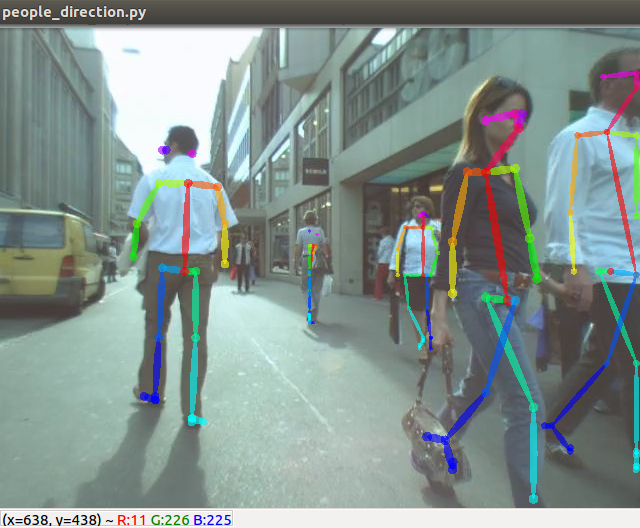
\includegraphics[width=1.0\linewidth]{img/chapter5_implementation/openposeKP.png}
        \caption{Key-point estimation is most accurate on people close-up.}
    \end{subfigure}%
    \hspace{\fill} 
    \begin{subfigure}[b]{.32\textwidth}
        \centering
        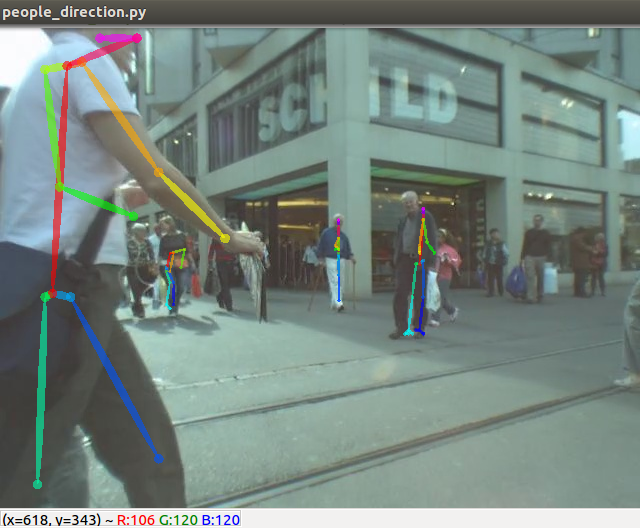
\includegraphics[width=1.0\linewidth]{img/chapter5_implementation/openposeKP1.png}
        \caption{On people at a distance, the estimation accuracy is limited by the network resolution.}
    \end{subfigure}
    \hspace{\fill} 
    \begin{subfigure}[b]{.32\textwidth}
        \centering
        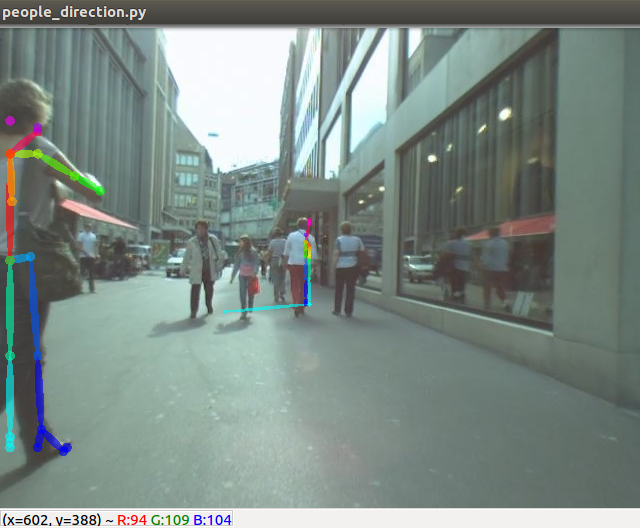
\includegraphics[width=1.0\linewidth]{img/chapter5_implementation/openposeKP2.png}
        \caption{A low network resolution results in difficulty discerning between people.}
    \end{subfigure}
    \vspace{-1\baselineskip}
    \begin{center}
        \caption{Comparison of keypoint estimation at different scales}
        \label{fig:openposeKP}
    \end{center}
        \vspace{-1.5\baselineskip}
\end{figure}

We highlight the issues in Figure \ref{fig:openposeKP}. The reason for the decrease in accuracy for people further away is due to the lower network resolution. Using a higher resolution allows us to detect people further away, but the delay between the arrival of the frame and the detection is more than 0.5 seconds. As such, to achieve real-time operation, we chose to use a lower network resolution.

\subsubsection{Defining Direction} \label{sec:keypointEstimate}
By comparing the relative positions of certain key-points, we can determine if a person is facing the camera or if they are walking away. This information is important since it will allow for better visualization of where a person is walking since people tend to walk in the direction they are facing. This also partially solves the direction problem brought up in Section \ref{sec:objecTrackingDirection}.

\begin{figure}[ht]
    \begin{subfigure}[b]{.32\textwidth}
        \centering
        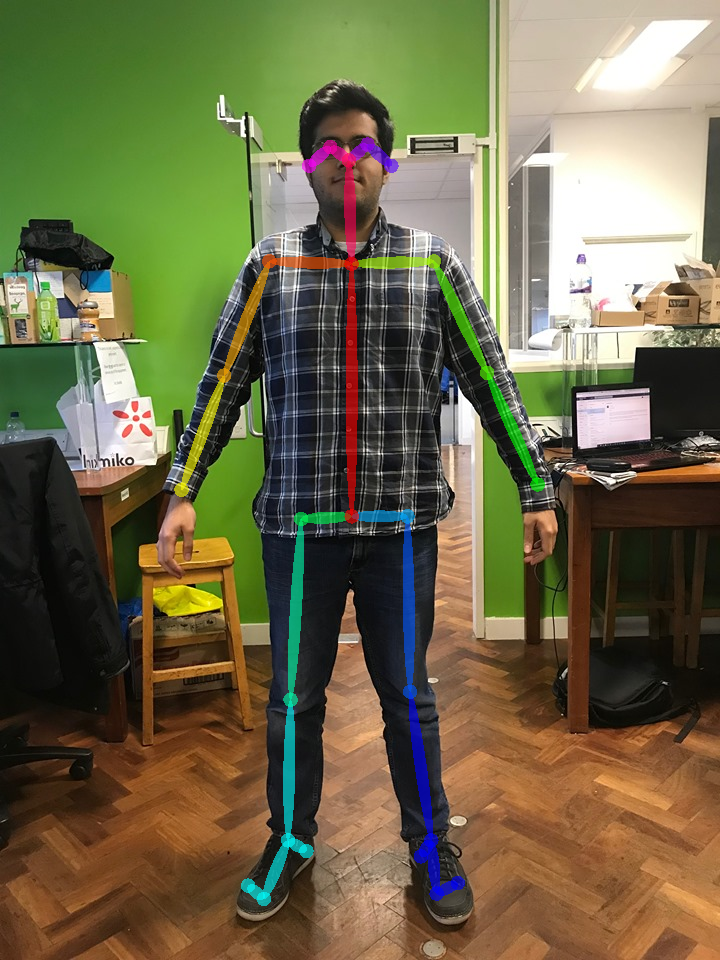
\includegraphics[width=1.0\linewidth]{img/chapter5_implementation/shreyFront.png}
        \caption{Frontal View}
    \end{subfigure}%
    \hspace{\fill} 
    \begin{subfigure}[b]{.32\textwidth}
        \centering
        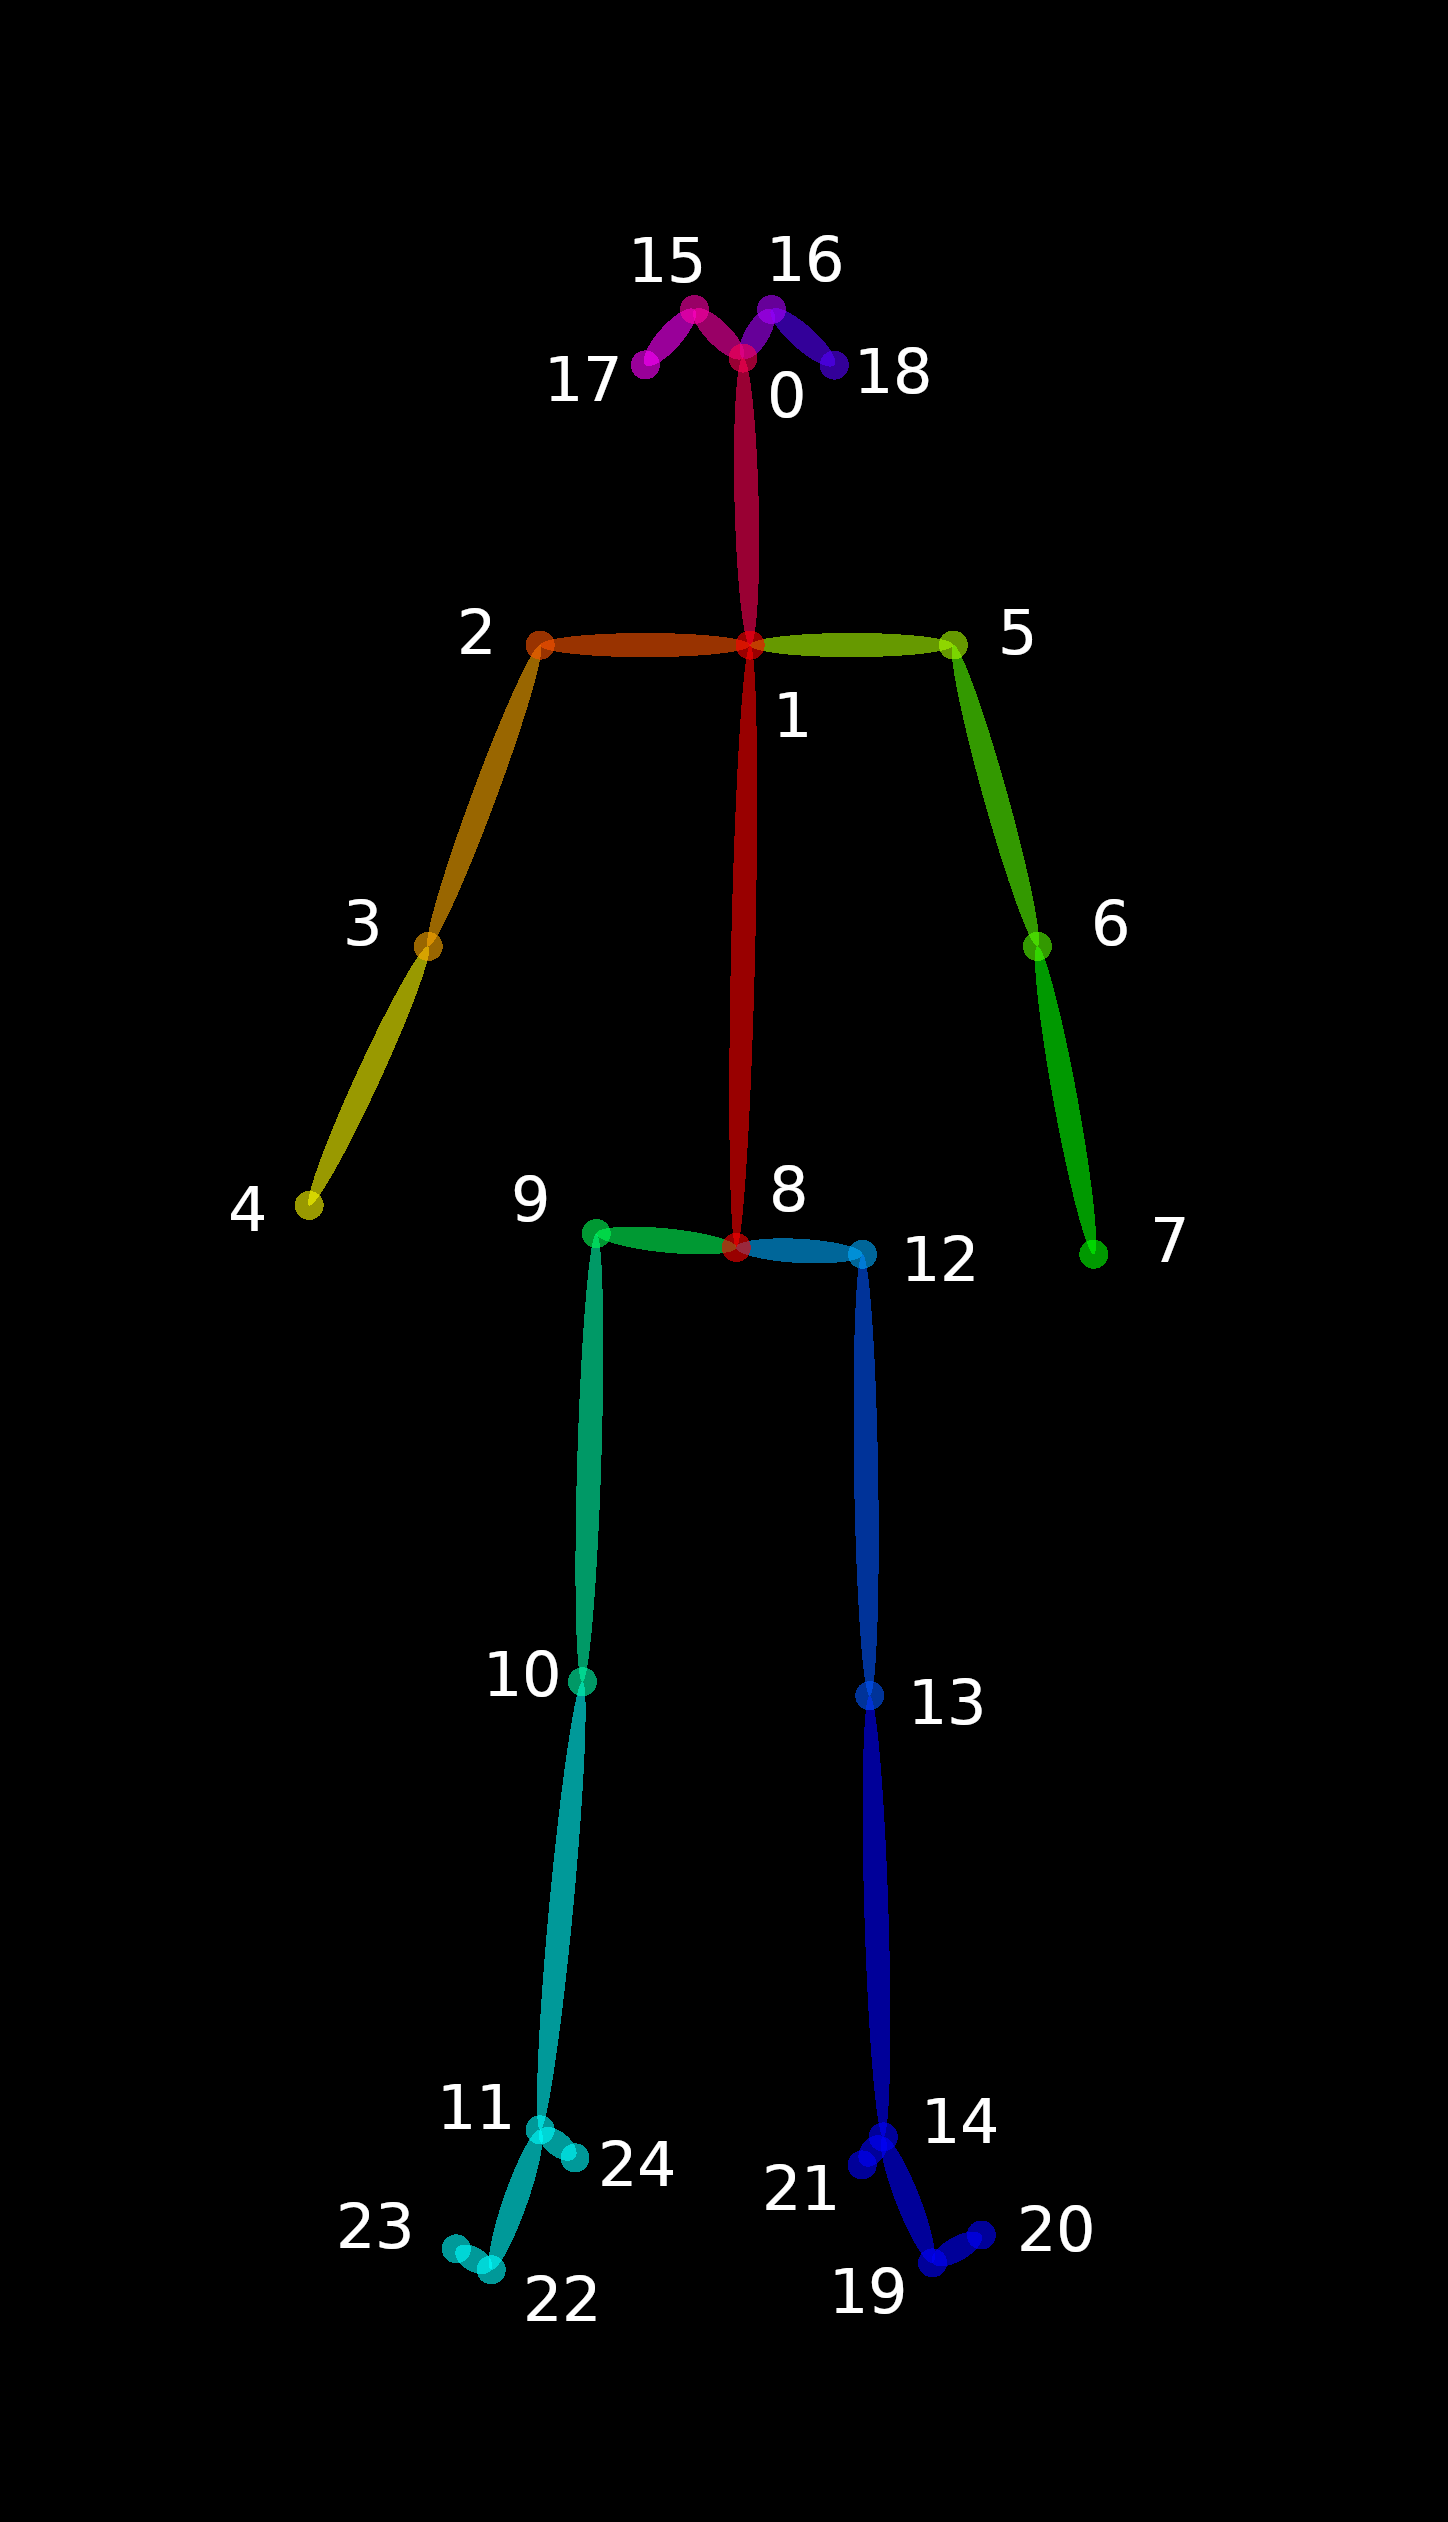
\includegraphics[width=0.765\linewidth]{img/chapter5_implementation/keypoints_pose_25.png}
        \caption{Key-point References}
    \end{subfigure}
    \hspace{\fill} 
    \begin{subfigure}[b]{.32\textwidth}
        \centering
        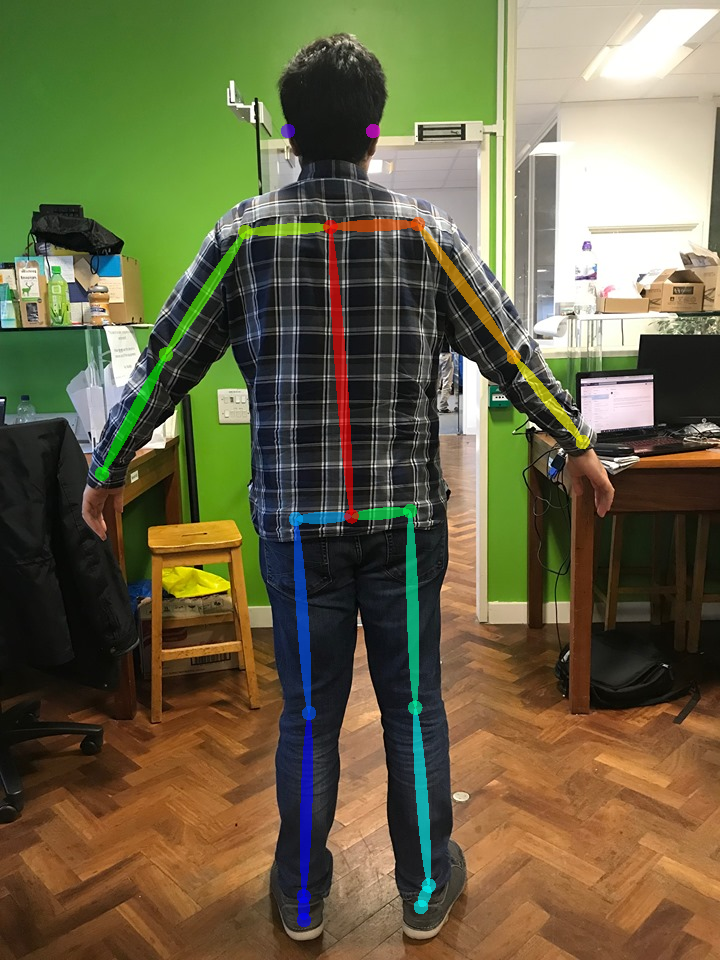
\includegraphics[width=1.0\linewidth]{img/chapter5_implementation/shreyBack.png}
        \caption{Back View}
    \end{subfigure}
    \vspace{-1\baselineskip}
    \begin{center}
        \caption{Body keypoint estimation of different views. These images show that the network can differentiate between left and right limbs.}
        \label{fig:keypointShrey}
    \end{center}
    \vspace{-2\baselineskip}
\end{figure}

\paragraph{Method} Pixels are measured from the top left corner of the image, with the x-axis extending horizontally to the right and the y-axis extending downwards. Figure \ref{fig:keypointShrey}.b shows the keypoint references for the body. The model can differentiate between the left and right limbs on a person. Figure \ref{fig:keypointShrey}.(a,c) show a full frontal and back keypoint detection on a person in the ideal detection position. 

\begin{table}[ht]
    \centering
    \begin{tabular}{|l|l|}
        \hline
        Body Part  & Key Points \\ \hline
        Right Arm  & 2, 3, 4    \\ \hline
        Left Arm   & 5, 6, 7    \\ \hline
        Head/Spine & 0, 1, 8    \\ \hline
    \end{tabular}
    \caption{Significant key-points for determining whether a person is facing the camera.}
    \label{tab:keypoints}
    \vspace{-1\baselineskip}
\end{table}

We can use the ability to differentiate between the left and right arms to determine if a person is facing the camera. Table \ref{tab:keypoints} presents the key-points for the relevant body parts. If the image co-ordinates of the left shoulder is further along the x-axis than the right shoulder, we can predict the direction as facing towards the camera. From testing, we know this simple method works most of the time. However, problems arise when a person is standing perpendicular to the camera. OpenPose has trouble detecting the torso and predicting the positions of the limbs, and it becomes difficult to decide if they are facing left or right.

\subsubsection{Implementation \& Detection Matching}
As mentioned in Section \ref{sec:bottomUp}, OpenPose uses a bottom-up approach by detecting individual body parts across the whole image. We need to match the OpenPose keypoint predictions with existing bounding boxes from YOLO since the tracker node assigns these detections a tracking ID. This is done in Listing \ref{lst:matchDetPose} \\

\begin{lstlisting}[language=Python, caption={Direction and Detection Matching code in people\_direction.py}, label={lst:matchDetPose}]
def matchDetectionAndPose(self, detections, poses):
    for pose in poses:
        # Check torso, right/left shoulder
        torso, rshoulder, lshoulder = pose[1], pose[2], pose[5]

        for bbox in detections:
            if( self.withinBB(bbox, torso[0], torso[1]) or
                self.withinBB(bbox, rshoulder[0], rshoulder[1]) or
                self.withinBB(bbox, lshoulder[0], lshoulder[1])):
   
                if(rshoulder[0] > lshoulder[0]):
                    directionTowardsCamera = False
                else:
                    directionTowardsCamera = True

                publishDetectionDirection() 
                break # Once matched, move onto next pose 
\end{lstlisting}

\vspace{-1\baselineskip}

\subsubsection{ROS Topic} \label{sec:yachtDirROS}
The direction node publishes the bounding box and direction to the Hololens. The \code{BoundingBox} data structure is defined in Listing \ref{bbmsg}, and is the same bounding boxes generated by the YOLO detector. \\

\begin{lstlisting}[language=Mymatlab,caption={ROS message structure for BoundingBoxDirection.msg}]
BoundingBox boundingBox
bool        directionTowardsCamera
\end{lstlisting}

\newpage
\section{Hololens Unity Application}
The Hololens is the central device in the overall system, acting as an intermediary between the HDD system and ARTA. We rely on the AR capabilities of the device to render visualization holograms to indicate to the user potential collisions. The depth camera and other sensors are used to perceive the distance of detected objects which are communicated to ARTA for reactive assistance. Most importantly, the front facing camera is the main visual input for the whole system, beginning the whole image processing pipeline. Without a live video stream from the camera, object detection and direction inference would be impossible. As such, the initial phase of the project was dedicated to producing a reliable video stream to an external computer. Figure \ref{fig:detailedHololens} shows the two separate parts of the Hololens application, the camera stream, and the holographic world. 

\begin{figure}[ht]
    \centering
    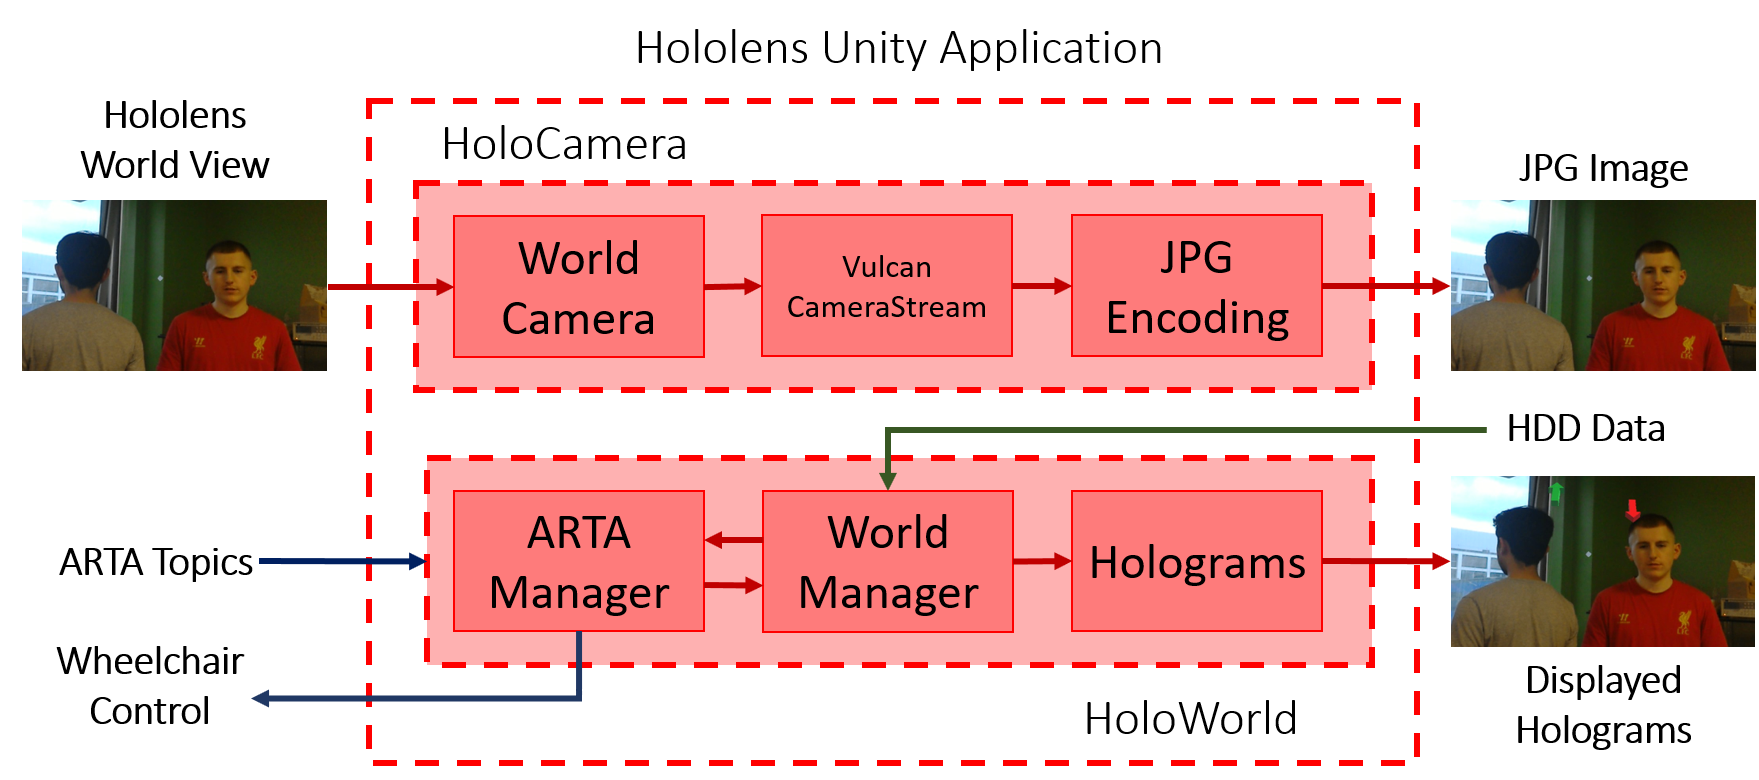
\includegraphics[width=1.0\linewidth]{img/chapter5_implementation/hololensSystemDiagram.png}
    \caption{Components of the Unity application running on the Hololens. We divide the program into two sub-programs, HoloCamera and HoloWorld.}
    \label{fig:detailedHololens}
\end{figure}

\paragraph{} Due to the importance, we begin this section by describing the implementation of the video camera stream. We explain the libraries used, the workarounds required to produce the stream, and the limitations of using a Unity-based approach. Afterwards, we describe the Unity application responsible for creating holograms, controlling ARTA, and how detected objects are placed in the Unity world. Finally, we explain the interaction between the Hololens and ARTA.

\subsection{Hardware \& Software Dependencies}
\subsubsection{Hardware}
\paragraph{Microsoft Hololens} The Microsoft Hololens is the world's first fully untethered holographic computer. The device can render 3D holograms in the world surrounding the user by displaying them on a set of see-through holographic lenses. The device is equipped with a multitude of sensors which we outlined in Section \ref{back:holo}. The device also supports gesture recognition for controlling the device, as well as voice input. The device is also able to connect to Wi-Fi networks, allowing it to stream data to and from other devices. We provide a complete device specification in the Appendix.

\begin{figure}[ht]
    \begin{subfigure}[b]{.45\textwidth}
        \centering
        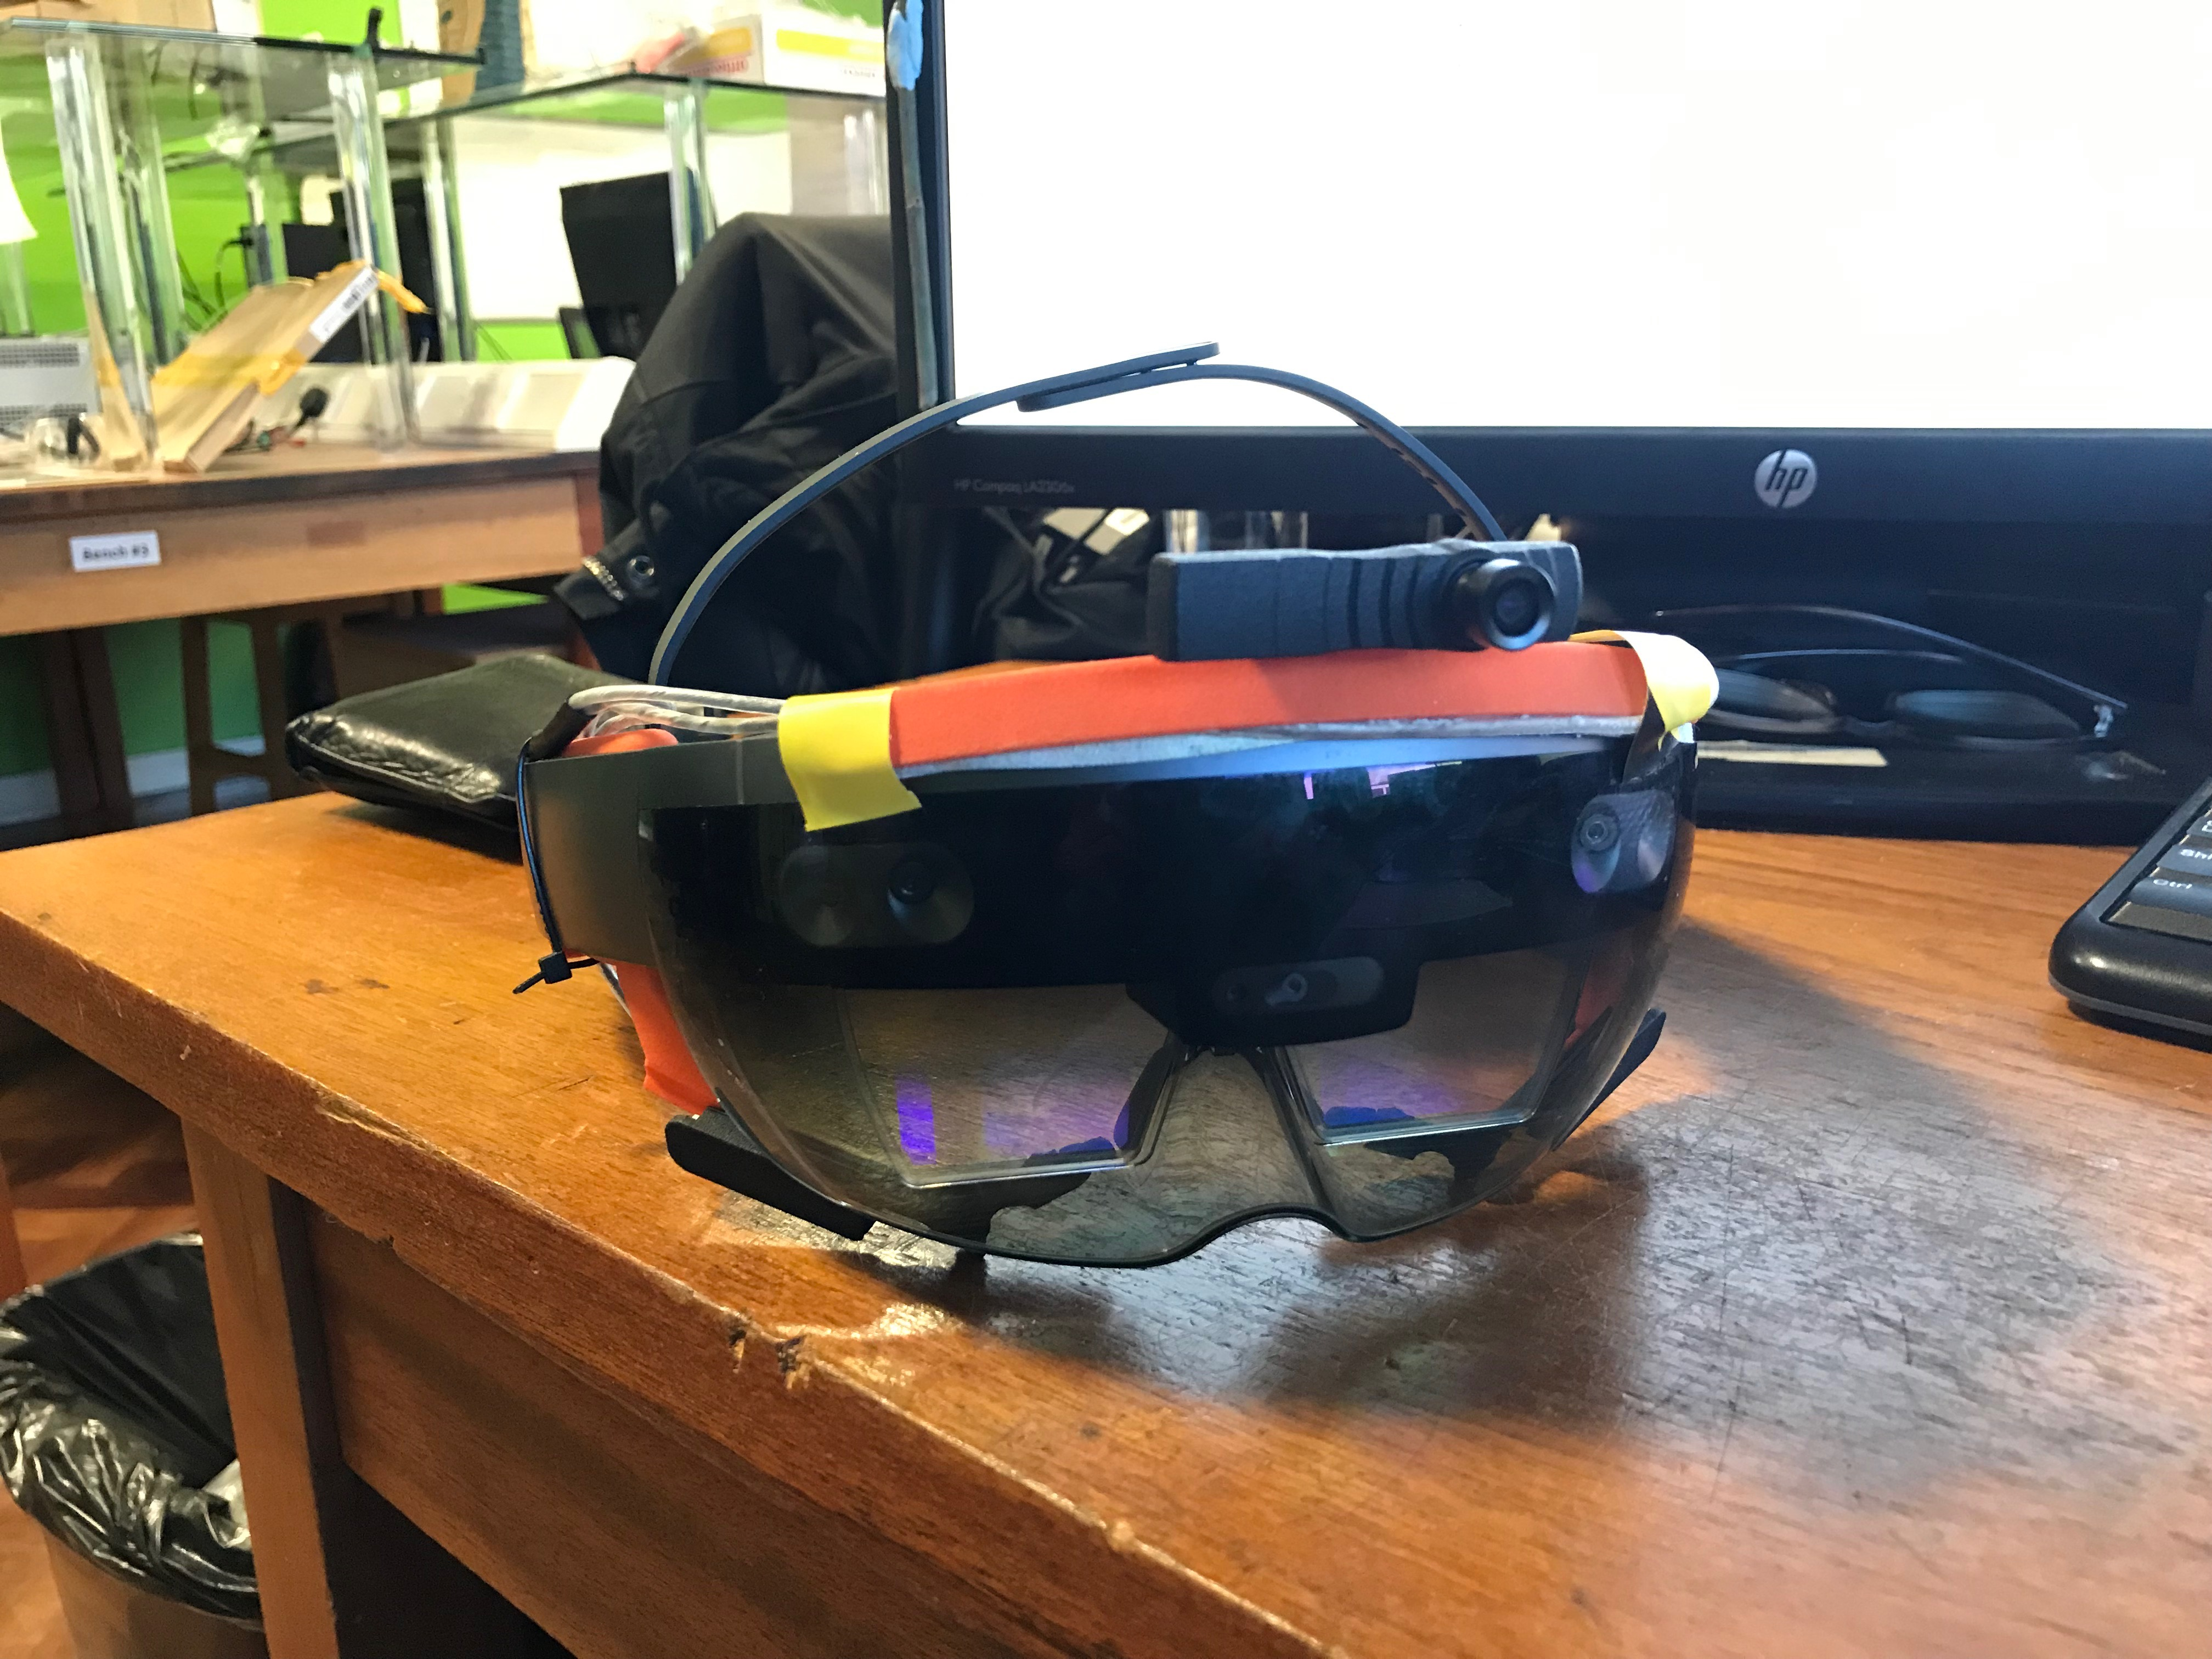
\includegraphics[width=1.0\linewidth]{img/chapter5_implementation/hololensDevice.jpg}
        \caption{The Microsoft Hololens with the see through holographic lenses.}
    \end{subfigure}%
    \hspace{\fill} 
    \begin{subfigure}[b]{.45\textwidth}
        \centering
        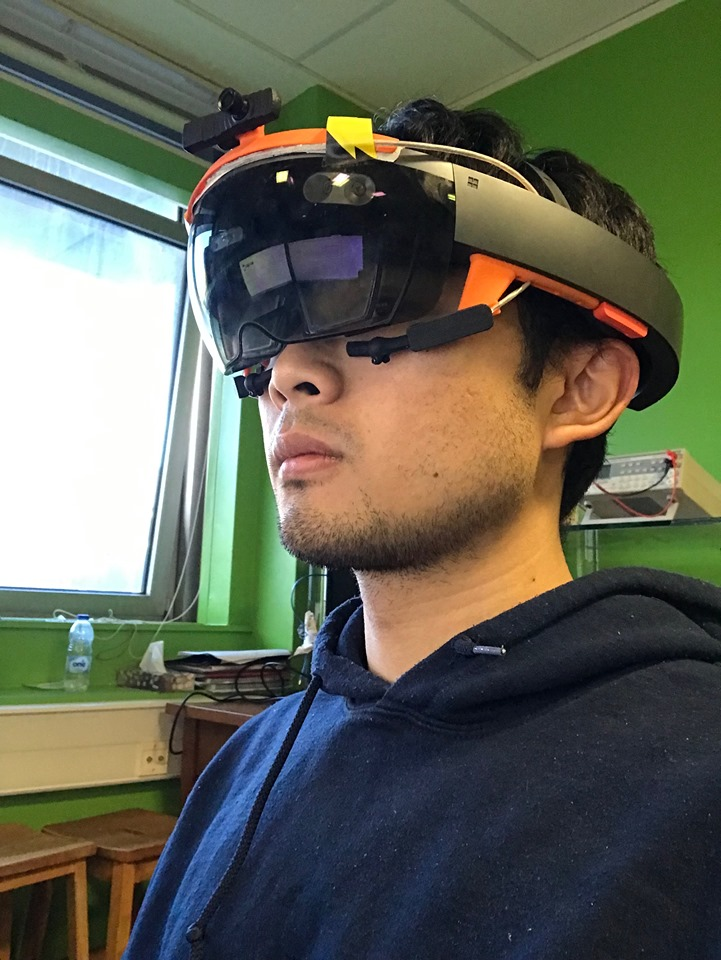
\includegraphics[width=0.55\linewidth]{img/chapter5_implementation/hololensOnHead.jpg}
        \caption{The device is worn on the head, resting on the bridge of the nose, similar to glasses.}
    \end{subfigure}
    \vspace{-1\baselineskip}
    \begin{center}
        \caption{The Hololens is larger compared to its competition. However, the increased number of sensors and wider spread usage makes it an ideal AR device for this project.}
        \label{fig:holodevice}
    \end{center}
    \vspace{-2\baselineskip}
\end{figure}

\subsubsection{Software}
\paragraph{Universal Windows Platform} The Universal Windows Platform (UWP) allows for applications that can be developed to run on any device running Windows 10. It gives the developer access to a set of standard APIs that make it easier to access data from any device. Software Development Kits (SDKs) are used to extend the capabilities of an app for specialized devices such as the Hololens.

\paragraph{Unity} Unity is a cross-platform game engine used to develop 3D, 2D VR \& AR visualizations for applications such as games, engineering or assistive robotics, among others. The primary programming language for the engine is C\#, and the engine has built-in Windows Mixed Reality and Hololens support, allowing for easier development of applications for the Hololens. 

\paragraph{Development Tools} For this project, we used the following setup for development:

\begin{itemize}
    \item Microsoft Hololens running Windows 10
    \item Laptop running Windows 10 Developers Fall Edition
    \item Unity Editor 2018.1.6f1 (64-bit)
    \item Visual Studio 2017 Community Edition
\end{itemize}

The application produced in the Unity Editor and Visual Studio 2017 is compiled and deployed to the Hololens as a UWP Unity application that can be accessed and run from the device's heads up display menu.

\subsection{Hololens Locatable Camera}
The images captured by the front facing camera is meant to be a representation of what the user is seeing. In reality, the field of view (FOV) of the front facing camera is greater than the actual FOV of the device, meaning the camera can see more of the world than the user can. 

\subsubsection{Specifications}
The front facing camera is a two megapixel photo/ HD video camera with auto white balance, auto exposure, and a full image processing pipeline. Due to the real-time requirement of the project, we chose to use the smallest video resolution possible in order to achieve the fastest frame rates. This limits the resolution of the captured video frames to $896\times 504$.

\subsubsection{Limitations} \label{sec:framerate}
The greatest limitation of the Hololens is the field of view. The FOV of the front facing camera is 48 degrees wide, allowing it to capture images of the surrounding world. However, compared to a standard mobile phone camera, the front facing camera provides a cut-off view of the world. We highlight this issue in Figure \ref{fig:holoVsIphone}, which shows the reduced FOV of the device. Another issue is that despite the image processing the pipeline, the Hololens camera produces overexposed images, especially when the front facing camera is pointed towards illuminating objects or when light is only coming from one direction. 

\begin{figure}[ht]
    \begin{subfigure}[b]{.45\textwidth}
        \centering
        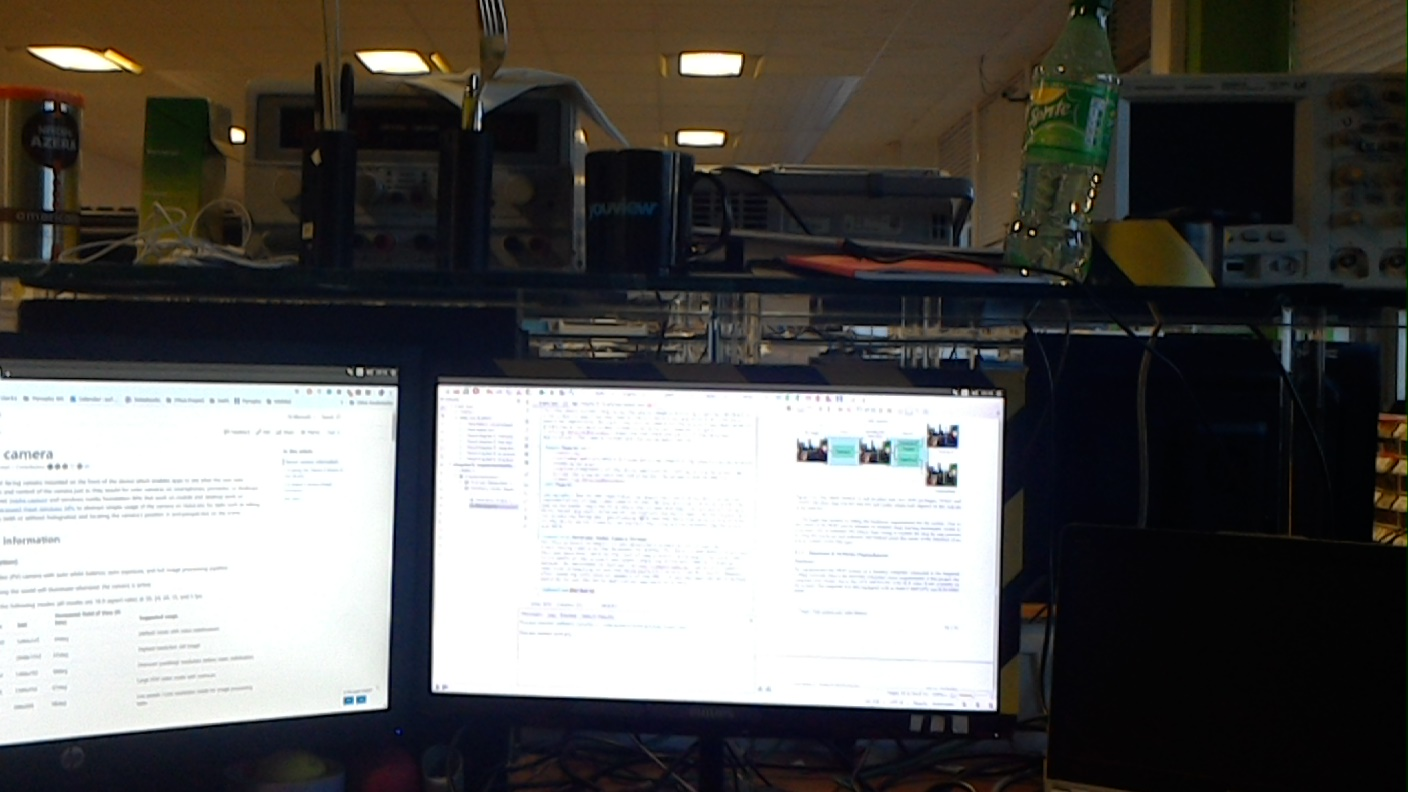
\includegraphics[width=1.0\linewidth]{img/chapter5_implementation/hololensFOV.jpeg}
        \caption{Image captured by Microsoft Hololens. Notice the overexposure in the image.}
    \end{subfigure}%
    \hspace{\fill} 
    \begin{subfigure}[b]{.45\textwidth}
        \centering
        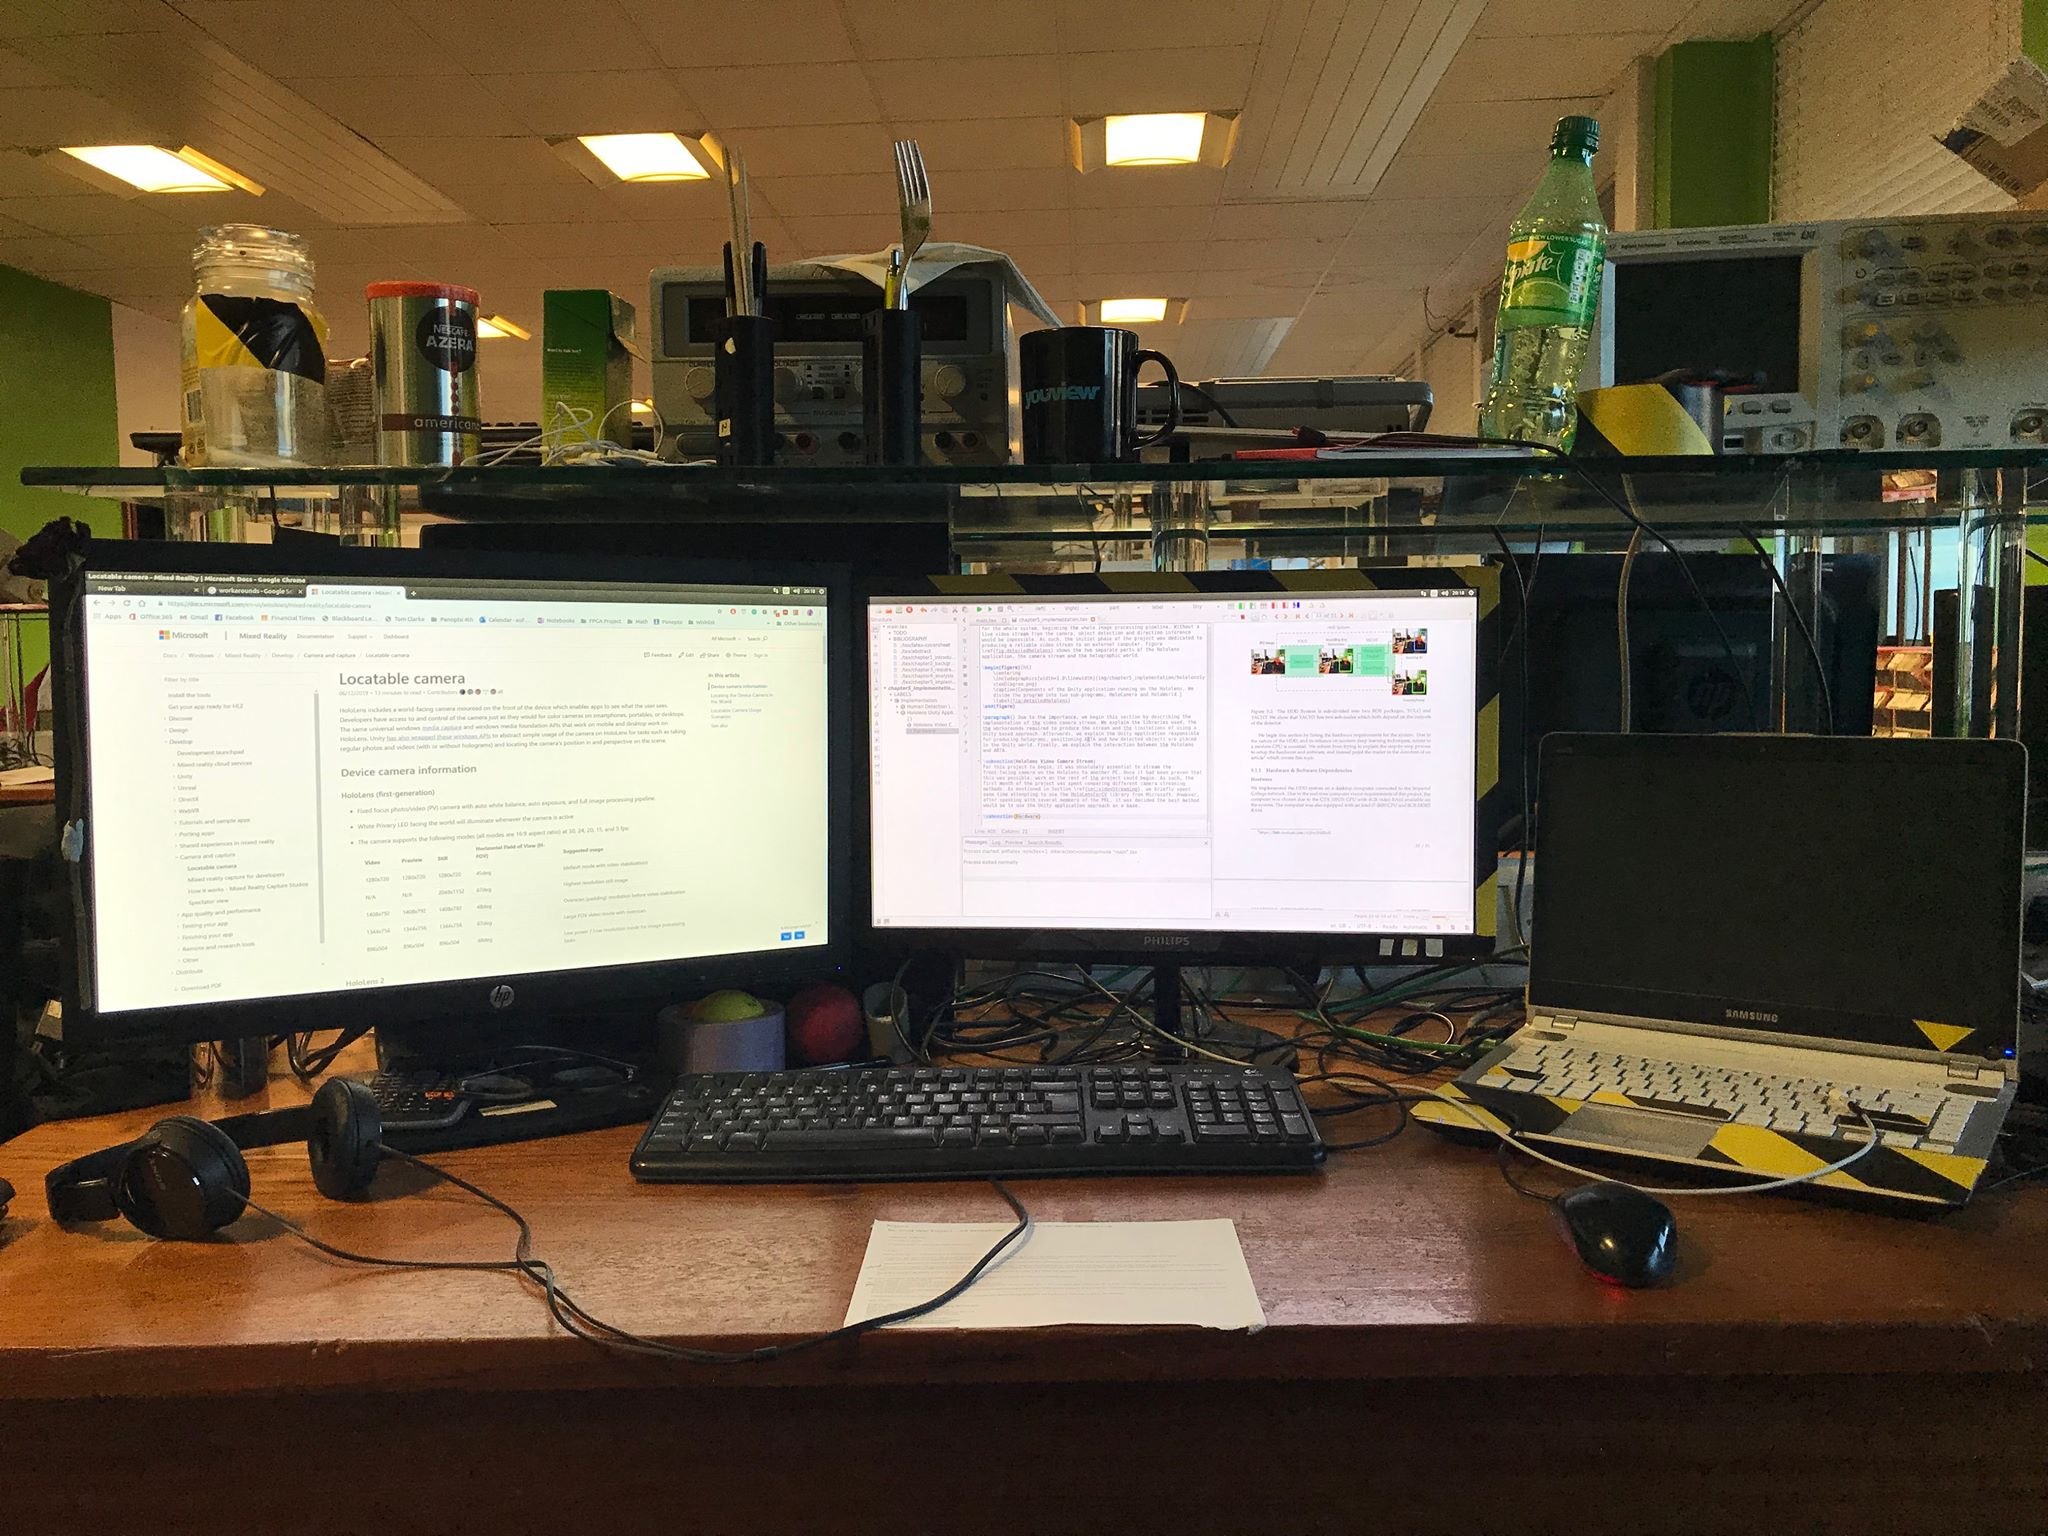
\includegraphics[width=1.0\linewidth,height=37.5mm]{img/chapter5_implementation/hololensFOVIphone.jpg}
        \caption{Image captured by standard IPhone Camera under the same light conditions.}
    \end{subfigure}
    \vspace{-1\baselineskip}
    \begin{center}
        \caption{These images were taken from the same position. The Hololens has a reduced FOV and is unable to capture the whole desk.}
        \label{fig:holoVsIphone}
    \end{center}
    \vspace{-2\baselineskip}
\end{figure}

Furthermore, due to the positioning of the holographic lenses, the users FOV is estimated to be approximately 29-30 degrees wide and 17 degrees high. This is even less than the front-facing camera and limits what the user can see in the surrounding area.

\subsection{Hololens Video Camera Stream}
For this project to begin, it was essential to stream the front-facing camera on the Hololens to another PC. Once it had been proven that this was possible, work on the rest of the project could begin. As such, the first month of the project was spent comparing different camera streaming methods. As mentioned in Section \ref{sec:videoStreaming}, we briefly spent some time attempting to use the HoloLensForCV library from Microsoft. However, after speaking with several members of the PRL, it was decided the best method would be to use the Unity application approach as a base.

\subsubsection{Image Capture}
The Unity engine on the Hololens has APIs for the front-facing camera, giving developers access to information such as the resolution of the captured images, the camera intrinsics, and the projection transform. However, Unity only allows developers to take a photo or video recording that is then saved onto the filesystem. The media can then be loaded from disk into Unity for streaming. This process is slow and time-consuming, due to the large overheads associated with writing media to and from disk. From experimentation, we deemed this method too slow for our use case and sought out an alternative.

\paragraph{Vulcan Technologies} HoloLensCameraStream is a Unity plugin\footnote{https://github.com/VulcanTechnologies/HoloLensCameraStream} developed by Vulcan Technologies that makes the Hololens front facing camera frames available inside the Unity app in real time. The original library was designed to give developers the ability to show a preview of what the Hololens camera sees within the application. The ability to access the raw frames inside saves the application from having to write the frame to disk and loading it again. Unfortunately, the library has not been maintained for newer versions of Unity with the last stable version being Unity 2017.3.1f . Furthermore, these older versions of Unity are incompatible with the ROS\# library we use to communicate with other ROS nodes. As such, we updated the plugin for Unity 2018.1.6f1 by modifying the offending code and updating obsolete functions to the newer 2018 Unity API.

\paragraph{Image Capture Pipeline} We briefly explain the image capture pipeline in the Unity application outlined in Figure \ref{fig:imgProcPipeline}. An instance of the updated Vulcan Technologies \textit{Camera Stream Helper} is added to the scene which provides access to the front facing camera video stream. We set the camera parameters to maximize the frame-rate by lowering the resolution. 

\begin{figure}[ht]
    \centering
    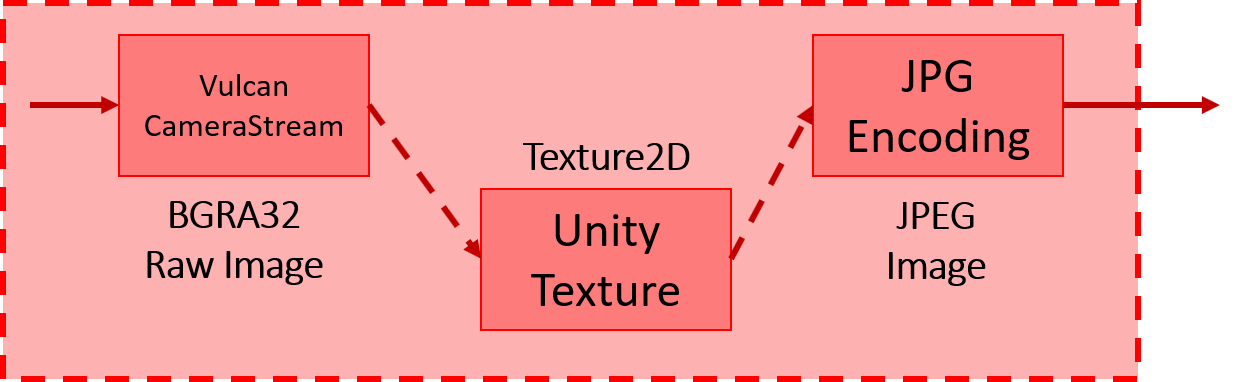
\includegraphics[width=0.6\linewidth]{img/chapter5_implementation/imageCapturePipeline.png}
    \caption{The image capture pipeline involves an intermediate Texture2D Unity state.}
    \label{fig:imgProcPipeline}
\end{figure}

\paragraph{} The captured frames are in the Microsoft standard \code{BGRA32} pixel format, which has 32 bits per pixel. The four channels (blue, green, red, and alpha) are each allocated 8 bits per pixel. The raw pixel format creates large filesizes unsuitable for streaming over the network. As such, it becomes necessary to compress the images into a PNG or JPEG format. Unity can convert \textit{textures}, a data structure for rendering images inside applications into a compressed image format to be saved to disk. We leverage this ability to compress the raw BGRA32 bytes into a JPEG image ready for network transfer.

\subsubsection{Image Compression}
Unity has built-in image compression techniques for saving textures to disk. JPEG images are generated through a lossy compression technique. The degree of compression can be adjusted, allowing a trade-off between image quality and storage size. Since these images are to be streamed over the network, we want to limit the size of the files not to use too much bandwidth. On the other hand, we want the quality of the image to be high enough so that we can conduct image processing in the HDD system. Through experimentation, we chose to set the image quality to 50\%, the middle ground between quality and filesize.

\paragraph{Unity Threading} Applications running on the Unity engine support threading, but due to many Unity types not being threadsafe, certain actions must be done in the main thread of the application. The main thread is responsible for all object interactions in the scene, as well as the rendering of holograms and other visualizations. On the other hand, tasks such as image capture by the Vulcan Camera Stream can be done in separate threads which are switched to from the main thread. We visualize the threading process in Figure \ref{fig:unityThreads}.

\begin{figure}[ht]
    \centering
    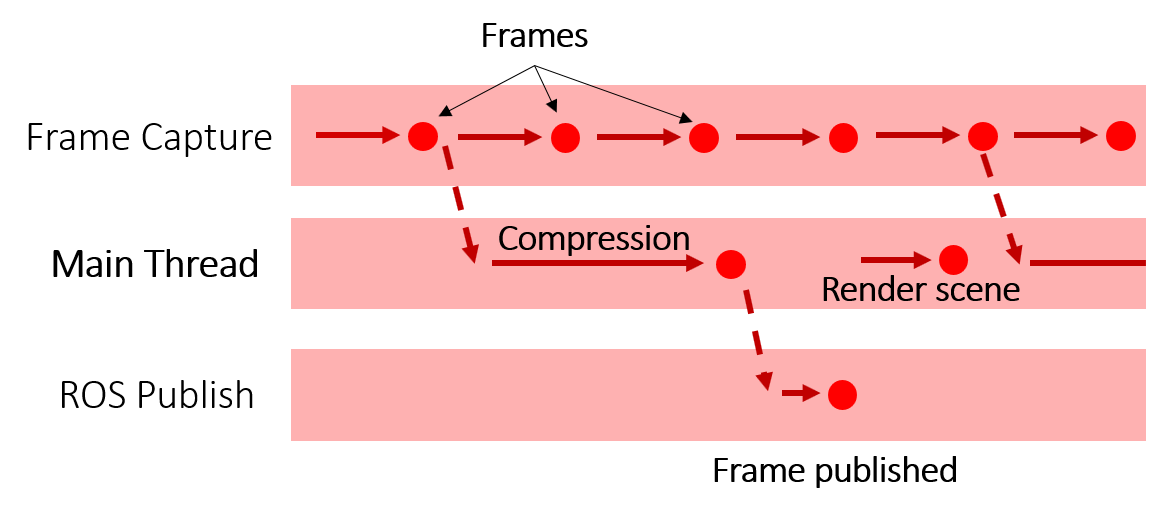
\includegraphics[width=0.8\linewidth]{img/chapter5_implementation/unityThreads.png}
    \caption{Image compression is a time consuming operation that must be done in the main thread. Only after compression is done can the holograms be rendered, limiting the application to 5 FPS.}
    \label{fig:unityThreads}
\end{figure}

\paragraph{Limited Frame-rate} An issue comes up with the way Unity implements image compression. The JPEG encoding reads the raw image bytes from a \code{Texture2D} object in the Unity scene. This action must be conducted on the main thread since updating textures involves object interactions. From code profiling, we determined that it takes approximately $0.2$ seconds to compress a captured frame. As such, the rendering of the scene can only be done after image compression. This results in a slight latency of the visualizations viewed by the PWU. 

\subsection{ROS Communication}
As explained in Section \ref{sec:rossharp}, we use the ROS\# library originally released by Siemens for our Unity to ROS communications. However, the original ROS\# library was not developed for Unity applications running on UWP. As such, we used a variant of the library\footnote{https://github.com/dwhit/ros-sharp} developed by David Whitney, a Ph.D. student at Brown University. 

\subsubsection{Modifications} The UWP version of ROS\# has been modified to only use APIs available on UWP devices such as the Hololens. Upon adding the ROS\# plugin to our Unity application, we encountered compatibility issues since the plugin was developed for Unity 2018.2 and above. We were forced to use 2018.1.6f1 since it is the most recent version of Unity, where the HoloCameraStream library works, and it is possible to access the camera frames inside the Unity application. As such, we had to backport the ROS\# library by changing function calls to newer API features not available in our version of Unity.

\subsubsection{ROS Topics}

\begin{figure}[ht]
    \centering
    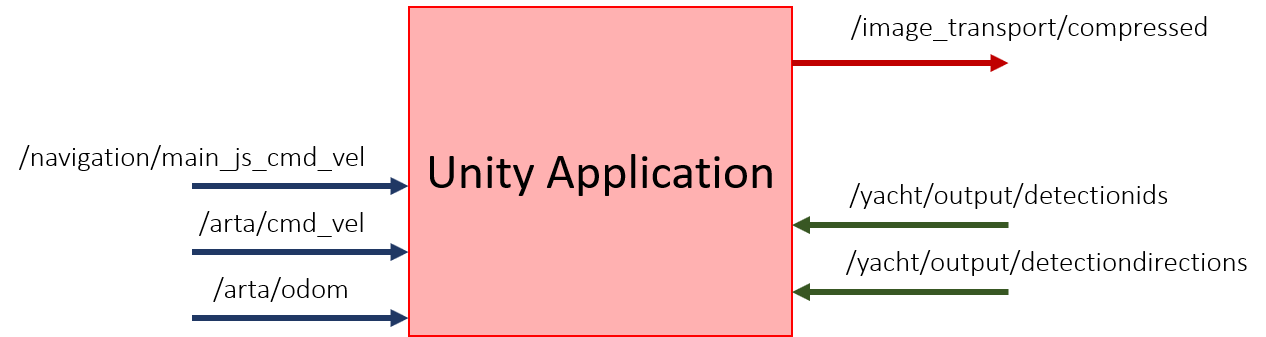
\includegraphics[width=1.0\linewidth]{img/chapter5_implementation/holoROSTopics.png}
    \caption{ROS topics in and out of the Unity application. Each topic carries data used by different parts of the overall system.}
    \label{fig:unityComms}
\end{figure}

\paragraph{Compressed Images} The raw video frames captured by the front-facing camera are compressed into JPEG frames that get published in the form of \code{CompressedImage} messages across ROS topics. Within the Unity application, we have setup \code{CompressedImage} publishers which are called when a compressed video frame is ready to be read into a message and published.

\paragraph{HDD Topics} In Section \ref{sec:yachtTrackROS} and Section \ref{sec:yachtDirROS}, we have explained the ROS messages published by the HDD system. The Hololens Unity application subscribes to these topics and receives the messages to transform the image co-ordinates into real world positions.

\subsection{Hololens World}
Mixed reality applications can place holograms in the world on real objects. This involves precisely positioning the holograms in places in the world that are meaningful to the user, which in the case of this project, is on detected people walking in the surroundings. Upon receiving messages from ARTA and the HDD system, the Hololens must parse the data to be able to update its internal understanding of the surrounding world. This section explains the other half of the Unity application, which is responsible for communication between devices, positioning of objects in the surrounding world, and visualizing detections using holograms.

\subsubsection{Hololens World Manager} \label{sec:holoworld}
Every Unity application has \textit{scenes} where developers can place \textit{GameObjects} which render holograms, recognize gestures, and communicate with other devices. A scene can be thought of as the Hololens' understanding of the world around it. The World Manager acts as the main program in the scene, receiving messages from the HDD system and ARTA, keeping track of objects in the surroundings and the position of the Hololens and ARTA in the real world.

\paragraph{Communication} The World Manager maintains a collection of all the publishers and subscribers on the Hololens. Figure \ref{fig:unityComms} outlines the flow of information in and out of the Unity application. By maintaining a central communication hub, specialized scripts such as the Hologram Manager or ARTA Manager can communicate with the other devices without having to create publishers or subscribers.

\paragraph{Spatial Mapping} Through spatial mapping, surfaces can be detected and objects rendered on top of tables or other solid objects. The Hololens has built-in cameras that continuously scan the surrounding environment, building up a virtual world geometry of the real world objects. The World Manager provides a central spatial mapping class that all scripts can access so they have the same understanding of the surrounding world.

\subsubsection{HDD Data to GameObjects} 
From Figure \ref{fig:unityComms}, we can see that the Unity application subscribes to two topics from the HDD system:

\begin{itemize}
    \item \code{/yacht/output/detectionids/}
    \item \code{/yacht/output/detectiondirections/}
\end{itemize}

These are the outputs of the two YACHT nodes described in Section \ref{sec:YACHT}, where we also describe the format of the output messages. The frames captured by the Hololens are sent to the HDD to be processed. From the frames, the HDD replies to the Hololens by sending bounding box image coordinates of the detections, as well as a tracking ID and whether the detected person is facing the camera.

\begin{figure}[ht]
    \centering
    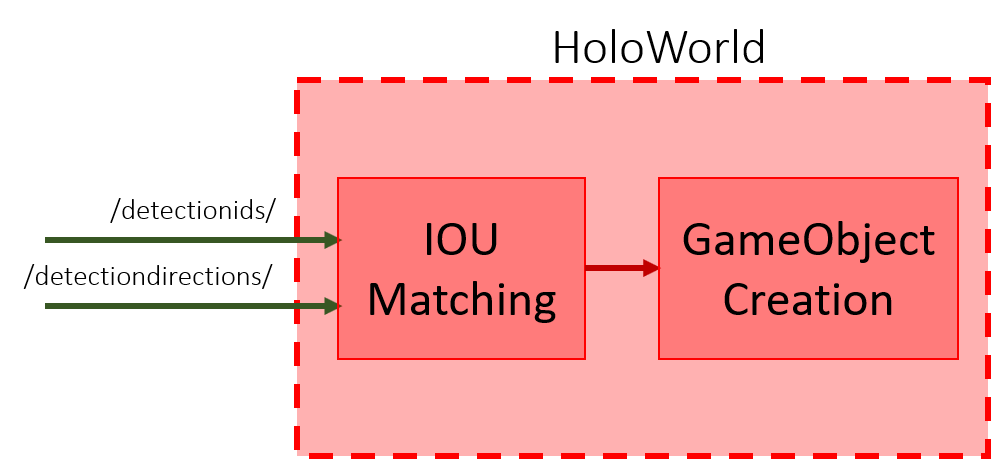
\includegraphics[width=0.9\linewidth]{img/chapter5_implementation/holoworldbreakdown.png}
    \caption{The Intersection-over-Union metric is used to compare bounding boxes for matching. The higher the metric, the more overlap between the boxes.}
    \label{fig:ioumatching}
\end{figure}

\paragraph{Matching Bounding Boxes} Due to the design of the YACHT package, two different nodes determine the tracking ID and direction of a detection. This allows the processing to be done in real-time by running on separate threads. Since both YACHT nodes subscribe to the bounding box detections from the YOLO node, we can match IDs and directions by comparing the bounding boxes contained in each message. \\

\begin{lstlisting}[language={[Sharp]C},caption={IOU metric C\# implementation}]
private float IntersectionOverUnion(BoundingBox a, BoundingBox b)
    {
        int xmin = Math.Max(a.xmin, b.xmin);
        int ymin = Math.Max(a.ymin, b.ymin);
        int xmax = Math.Min(a.xmax, b.xmax);
        int ymax = Math.Min(a.ymax, b.ymax);

        int interArea = Math.Max(0, xmax - xmin + 1) * Math.Max(0, ymax - ymin + 1);

        int aArea = (a.xmax - a.xmin + 1) * (a.ymax - a.ymin + 1);
        int bArea = (b.xmax - b.xmin + 1) * (b.ymax - b.ymin + 1);

        float iou = interArea / (float)(aArea + bArea - interArea);

        return iou;
    }
\end{lstlisting}

We use the Intersection-over-Union (IOU) metric to match the bounding boxes by comparing the amount of overlap. This was done since there may potentially be network delays between the received messages. If latency is involved, the bounding boxes from the detection may not match up precisely, since one message may be compared with another message from the frame before. By using IOU, we can compare the metric to a threshold to determine a match.

\paragraph{Creating GameObjects} We use GameObjects to represent the detected people in the surroundings. Before we can place the GameObjects of the people in the scene, we first need to determine the real world positions from the position in the image frame. This is done by un-projecting the image and using a coordinate frame transforms to convert the point in the Camera coordinate system to the World coordinate system. We highlight the process in Figure \ref{fig:cameraProjection}.

\begin{figure}[ht]
    \centering
    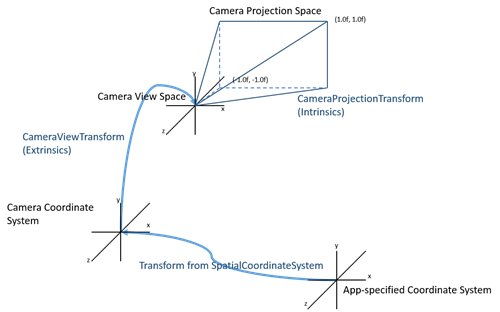
\includegraphics[width=0.8\linewidth]{img/chapter5_implementation/CameraTransform.png}
    \caption{The front facing camera projects the surroundings onto a 2D plane. We can determine the real world position of a pixel by reversing the projection and using frame transforms.}
    \label{fig:cameraProjection}
\end{figure}

Fortunately, the Vulcan Technologies library used to capture the frames has a function that converts pixel locations to world space coordinates. Using the \code{camera2World} matrix transform and camera projection matrix, the \code{PixelCoordToWorldCoord()} function determines the real world position of a pixel. We use the centre of the bounding box centres to represent the position of the detected people, and we place the GameObjects at the initial world space position determined by the function.

\subsubsection{Hologram Manager}
The Hologram Manager is the manager of visualizations rendered on the holographic screens. The GameObjects representing detected people created by the World Manager are used to determine the initial positions of the holograms, but the Hologram Manager uses ray casting and spatial mapping to correct the positioning of the GameObjects. The holograms are then rendered by the manager in their correct positions to communicate to the PWU if people are walking towards them or not.

\paragraph{Holograms} We use \textit{prefabs}, 3D holographic models we created in the Unity editor to create the visualizations. When the GameObjects representing people are created, they are invisible to the PWU, since we are not rendering any textures on the objects. By attaching a prefab to the GameObject, we essentially place a hologram at the position of the GameObject in 3D world space. We have created two prefabs, a green and red arrow. The green arrow indicates to the PWU that the person is moving away or in the same direction as the PWU is facing, while a red arrow represents a person walking towards the PWU. We show these prefabs in Figure \ref{fig:holograms}, as well as the blue cursor that indicates to the PWU where they are looking.

\begin{figure}[ht]
    \centering
    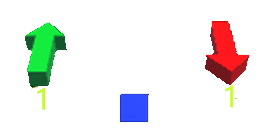
\includegraphics[width=0.5\linewidth]{img/chapter5_implementation/greenredholowhite.png}
    \caption{The Green and Red Arrow prefabs. The number under the arrow is the associated tracker ID of the object. This allows us to track objects in the surroundings.}
    \label{fig:holograms}
\end{figure}

To improve the positional accuracy of the holograms, we utilize the spatial mapping capabilities of the Hololens. By using the \code{Raycasting} function in Unity, we can project a ray from the Hololens in the direction of the GameObject. When the ray hits a surface detected by the spatial mapping class, we render the hologram on the surface and move the GameObject to that position. This tries to ensure that the holograms are rendered on the detected person, as seen in Figure \ref{fig:greenredrender}.

\begin{figure}[ht]
    \begin{subfigure}[b]{.45\textwidth}
        \centering
        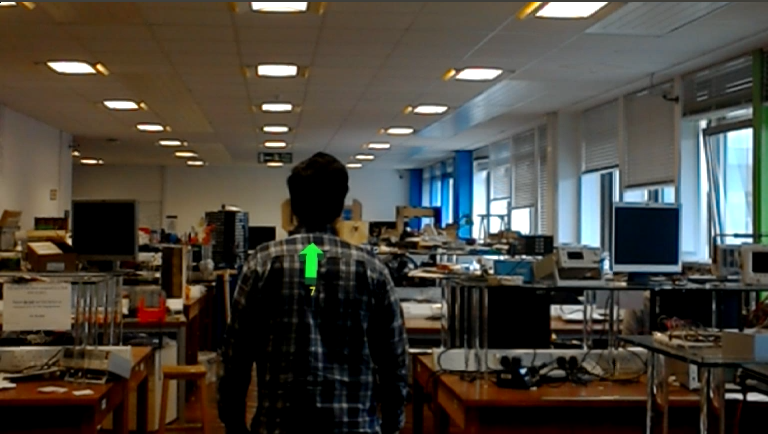
\includegraphics[width=1.0\linewidth]{img/chapter5_implementation/shreyAway.png}
        \caption{Green Arrow hologram rendered on a person walking away.}
    \end{subfigure}%
    \hspace{\fill} 
    \begin{subfigure}[b]{.45\textwidth}
        \centering
        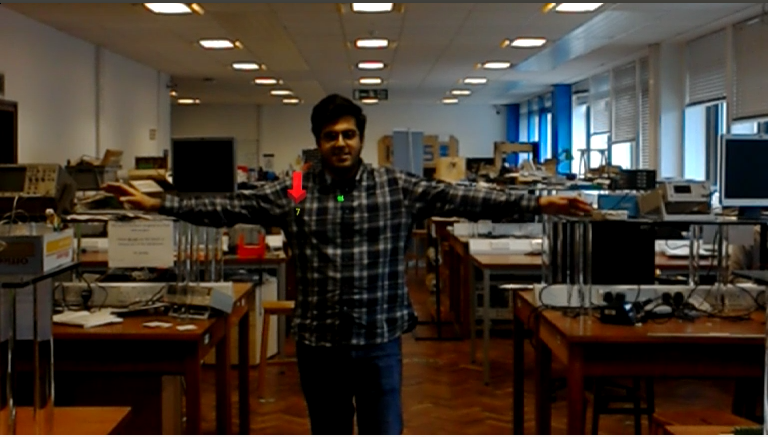
\includegraphics[width=1.0\linewidth]{img/chapter5_implementation/shreyCome.png}
        \caption{Red Arrow hologram rendered on a person walking towards the camera.}
    \end{subfigure}
    \vspace{-1\baselineskip}
    \begin{center}
        \caption{Images captured from the Hololens showing what the PWU would see when wearing the device.}
        \label{fig:greenredrender}
    \end{center}
    \vspace{-2\baselineskip}
\end{figure}

\subsubsection{ARTA Manager}
We create a GameObject to represent the powered wheelchair within the Unity application. The ARTA manager subscribes to topics published by the ROS nodes on the device, shown in Figure \ref{fig:unityComms}. Using the messages received from the powered wheelchair, it is possible for the application to understand the PWU's control intentions and to make decisions reactively. We explain the collision avoidance reactive control system in the next section of this report.

\section{ARTA Powered Wheelchair}
The Assistive Robotic Transport for Adults is a powered wheelchair developed by the Personal Robotics Lab at Imperial College London. A PWU can control the device through a joystick that converts the user issued commands into motor signals. We communicate the wheelchairs velocity and PWU control signals to the Unity application running on the Hololens and using the messages from the HDD system; we developed a reactive control system to detected people in the surroundings of the PWU. 

\begin{figure}[ht]
    \centering
    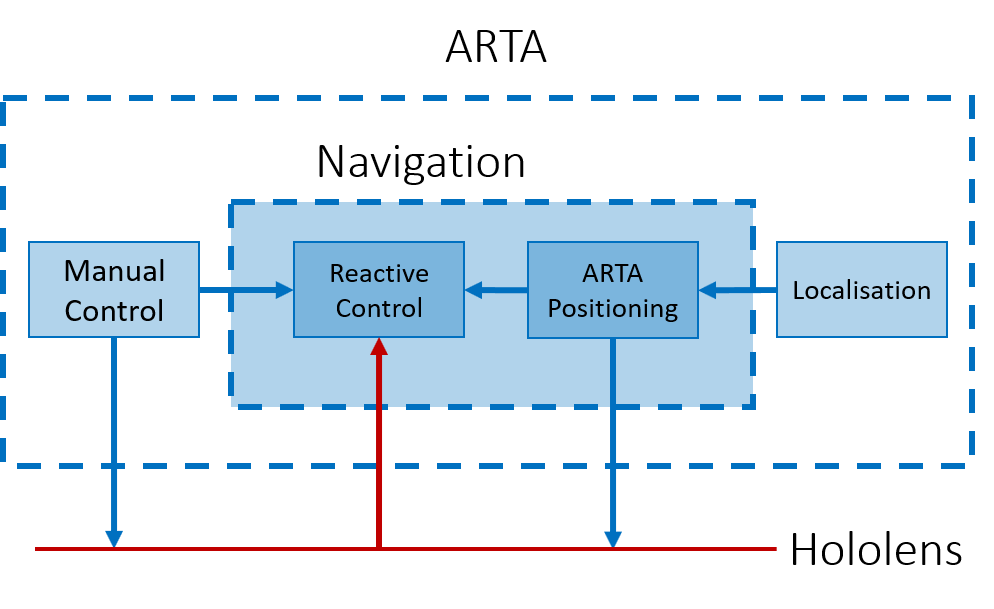
\includegraphics[width=0.8\linewidth]{img/chapter5_implementation/artaSystemDiagram.png}
    \caption{The ROS nodes running on ARTA. We utilize PRL ROS packages as a base and communicate with the Hololens for reactive control.}
    \label{fig:detailedARTA}
\end{figure}


\subsection{Hardware \& Software Dependencies}
Building a powered wheelchair with the required sensors for localisation and mapping is a time-consuming process, well beyond the scope of this project. We rely on the sensors already attached to the wheelchair, as well as the ROS packages developed internally for the conversion of joystick commands to control signals and communication between ROS nodes.

\subsubsection{Hardware}
The following sensors are fixed to the powered wheelchair for navigation and localization purposes. The laptop is used as the main control system running the ROS nodes that utilize the sensor data. 

\begin{itemize}
    \item Arduino Uno (Joystick to motor signal conversion).
    \item 2 Hokuyo URG-04LX-UG1 laser scanners.
    \item SICK LMS200 rangefinder.
    \item Phidgets spatial 3/3/3 IMU.
    \item Laptop running ROS nodes.
\end{itemize}

\subsubsection{Software}
The PRL has several GitHub repositories dedicated to the ROS nodes running on ARTA. These ROS packages cover the robotic aspect of the powered wheelchair, from using the sensor data for localization and mapping of the surroundings, to receiving control signals from the joystick or other exotic control interfaces. We utilize these repositories to build the base ARTA system that is needed to control the robot using the joystick.

\subsection{PRL ROS Packages}
A large robotic device, such as ARTA requires a lot of software to control. As such, the PRL has divided the ARTA functionality into several ROS packages, each responsible for a certain aspect of controlling the powered wheelchair. We utilize these packages as a base and contribute our additional reactive control module which works in conjunction with detections from the Hololens.

\subsubsection{ARTA}
The ARTA ROS package is the main parent node that encompasses the other packages we describe in this report. The package is responsible for the basic manual control and sensor node activation. It provides an interface via ROS messages for other nodes to communicate with, such as the localisation or navigation nodes. Furthermore, the package is responsible for the Gazebo simulation of the device, such as the model of the wheelchair and control systems.

\subsubsection{Localisation}
The PRL Localisation package is an internally developed library for the robots in the PRL lab. It contains various ROS launchers for common SLAM and localisation packages such as the \code{hector\_mapping} SLAM approach that utilizes laser scan data for mobile robots. The package also contains maps for use with the \code{amcl} package for localisation of the robots. The members of the PRL have constructed maps for commonly used testing areas, such as the hallway outside the PRL lab on the 10th floor of the EEE building. We leverage these pre-existing maps for testing and evaluation later in this report.

\subsubsection{Navigation}
In addition to the localisation package, the PRL has developed a ROS package for assistive navigation of the mobile robots in the lab. The package encompasses obstacle avoidance, autonomous navigation as well as shared control. Using the sensor data and localisation techniques from the other packages, we developed our reactive control system with this as a base.

\subsection{Hololens Communication}
As shown in Figure \ref{fig:unityComms}, the Hololens Unity application requires data from ARTA to build a Unity GameObject of the powered wheelchair. We utilize ROS topics and messages to communicate to the Hololens the position of the wheelchair in the world, the PWU's joystick input controls, and the current wheelchair velocity. Additionally, Figure \ref{fig:detailedARTA} shows the communication from the individual ARTA nodes and highlights the control messages received from the Hololens.

\subsection{Reactive Control}
The goal of this project was to build an augmented reality system that would assist PWU in their day to day navigation tasks. Detection of people in the surroundings and visualization of their direction is useful to the PWU, but reactive control for assistive navigation and object avoidance can be seen as a direct use of the people detection. We contribute a system that uses the people detection data from the HDD system and front-facing camera of the Hololens to manipulate the PWU manual control signals for wheelchair control.

\begin{figure}[ht]
    \centering
    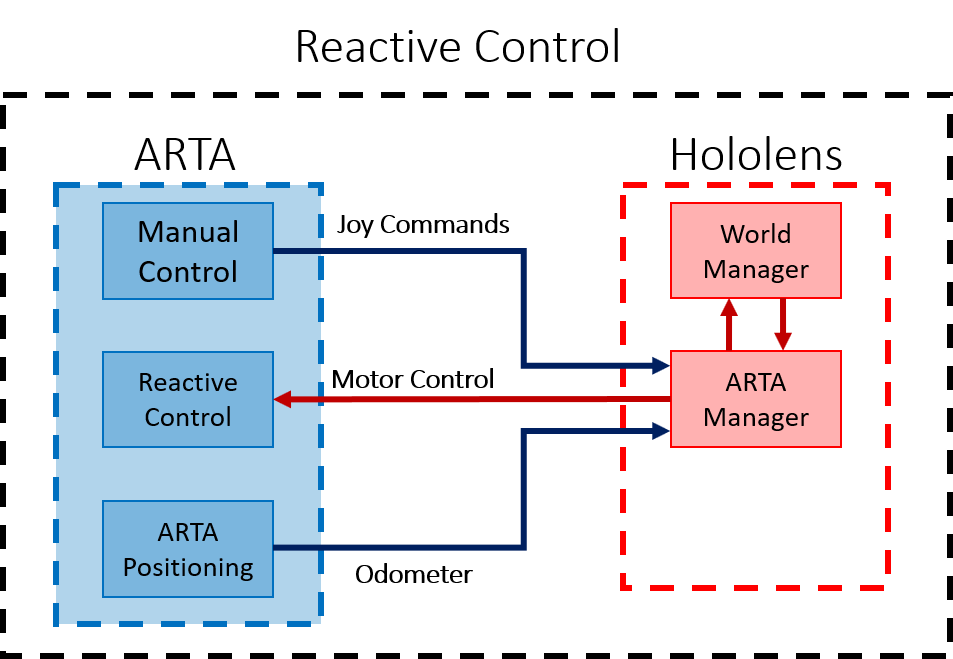
\includegraphics[width=0.6\linewidth]{img/chapter5_implementation/reactiveControlSystem.png}
    \caption{The Reactive Control system spans both ARTA and the Hololens, due to its dependency on ARTA sensor data as well as the Unity converted HDD system GameObjects.}
    \label{fig:detailedReactive}
\end{figure}

We have left the explanation of the reactive control system for last since it spans both ARTA, the Hololens Unity application. We go over the flow of information through the systems, how they contribute to the final reactive control decisions made by the ARTA manager on the Hololens and how it is translated to motor signals and movement of the powered wheelchair.

\subsubsection{ARTA}
\paragraph{Manual Control} The powered wheelchair is controlled using a joystick, which the PRL have attached a circuit board and Arduino UNO that converts the user inputs into control signals. The signals are published on the \code{/arta/arta\_joystick} topic, which are sent to the nodes responsible for turning the wheels on the device. Furthermore, the localisation and navigation nodes also subscribe to these topics, since libraries such as the obstacle avoidance nodes require the user input signals. As shown in Figure \ref{fig:detailedReactive}, the Hololens also subscribes to the topic via the ARTA manager.

\paragraph{ARTA Positioning} For this project, we have limited the scope to navigating the wheelchair in the hallway outside of the Personal Robotics Lab. We have chosen this since the PRL have already built up height maps of the hallway, allowing the localisation packages to determine the position of the wheelchair in the world accurately. By publishing the odometer readings to the Hololens, we can determine the rotation of PWU relative to their head rotation, solving the issue of not knowing if a detected person is directly in front of the wheelchair brought up in Section \ref{sec:alignment}.

\subsubsection{Hololens}
\paragraph{World Manager} As explained in Section \ref{sec:holoworld}, the World Manager creates GameObjects representing human detections in the Unity scene. By maintaining a map of the positions of these objects, the reactive control system can use spatial mapping to determine the distance between objects in the real world.

\paragraph{ARTA Manager} The ARTA manager forms the central part of the Reactive Control system. It subscribes to the control and odometer readings from the powered wheelchair and uses it to determine if a detected person is in front of the wheelchair and poses a collision risk. Furthermore, upon determining a risk, it manipulates the PWU control inputs to minimize the risk of a collision by lowering the speed of the wheelchair relative to the distance and direction of the person.

\subsubsection{ARTA Hololens Alignment}
As brought up in Section \ref{sec:alignment}, the major issue we are faced with is determining if a person detected by the Hololens is in front of the wheelchair, or if the PWU is looking to the side, and the person is not in the wheelchairs forward trajectory. We visualized this problem in Figure \ref{fig:holoArtaAlignment}, and show the alignment of the Hololens and ARTA frames in Figure \ref{fig:holoArtaFrames}.a. Although the PWU can tilt their head and rotate the Hololens about the x and y-axis, we have simplified the model and assumed that the PWU will only rotate about the z-axis. Furthermore, through testing, we have determined that the Hololens can only rotate around the z-axis between $-90$ and $+90$ degrees. The PWU is unable to swivel their head further, due to human biomechanics and the headrest of the wheelchair.

\begin{figure}[ht]
    \begin{subfigure}[b]{.45\textwidth}
        \centering
        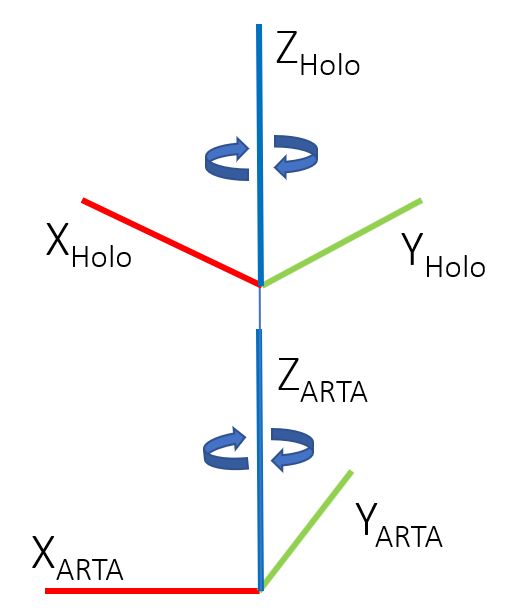
\includegraphics[width=0.75\linewidth]{img/chapter5_implementation/holoArtaFrames.png}
        \caption{The Hololens frame can rotate between -90 and +90 degrees, while ARTA can rotate 360 degrees.}
    \end{subfigure}%
    \hspace{\fill} 
    \begin{subfigure}[b]{.45\textwidth}
        \centering
        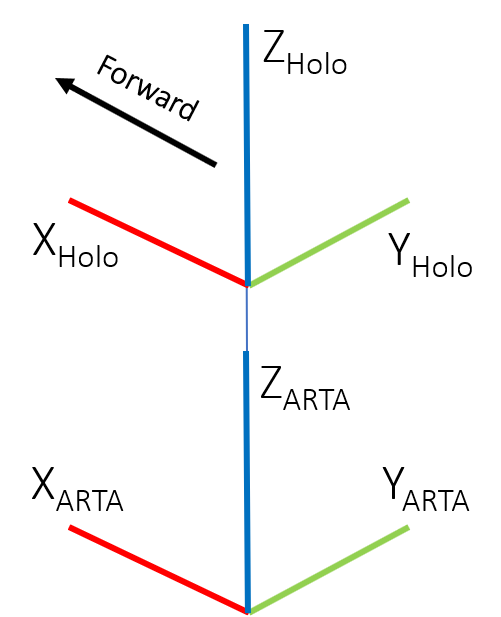
\includegraphics[width=0.75\linewidth]{img/chapter5_implementation/holoArtaFramesAligned.png}
        \caption{We calculate the offset between the Hololens and ARTA by aligning the frames during calibration.}
    \end{subfigure}
    \vspace{-1\baselineskip}
    \begin{center}
        \caption{The alignment of the ARTA and Hololens. We note that both frames can rotate about the z-axis.}
        \label{fig:holoArtaFrames}
    \end{center}
    \vspace{-2\baselineskip}
\end{figure}

However, ARTA is limited to rotations about the z-axis, since the powered wheelchair moves within the 2D plane of the floor. As such, we can determine the initial alignment between ARTA and the Hololens.

\paragraph{Alignment Process} Upon starting the Hololens Unity application and ARTA nodes, the Hololens subscribes to the odometry topic published by ARTA. By accessing the pose message contained within the odometry message, we can determine the orientation of the robot in space. The PWU wears the Hololens and sits in the powered wheelchair, facing directly forward. After 5 seconds, the ARTA manager aligns the Hololens to ARTA by calculating an offset between the current ARTA rotation and Hololens rotation measured by the IMU of the device. We show this alignment in Figure \ref{fig:holoArtaFrames}.b. This offset is used to determine whether the PWU is looking forward or to the side. 

\subsubsection{Unity Distance to Objects}
The World Manager uses spatial mapping and raycasting to correct the world positions of the GameObjects representing the detected people. The Hololens has an optimal hologram placement range of between $2$ meters and $5$ meters. This means after correction; we can be more certain about the distance to the GameObjects if they are within this range. Unity keeps an internal spatial coordinate system of the world, and by keeping track of the Arta/Hololens GameObject position, we can calculate the distance between the device and detected people in the scene.

\subsubsection{Reactive Control Algorithm}
The ARTA Manager subscribes to the PWU joystick inputs which are translated to ROS \code{Twist} messages. These messages represent the linear and angular velocities of the wheels of the powered wheelchair. The forward kinematics of the wheelchair is determined by the linear velocities of the left and right wheel of the wheelchair. To turn the wheelchair, we use angular velocities representing rotations in the z-axis. These messages are received by the Hololens and interpreted to determine the current trajectory of the wheelchair. 

\paragraph{} At the same time, the ARTA Manager searches through the Unity scene for GameObjects in front of ARTA/Hololens and groups them by the direction component of the GameObject from the HDD system. The reactive control system iterates over the GameObjects with directions coming towards the PWU first, since these are more likely to cause a collision. The system then calculates the distance between the PWU and the detected person. 

\begin{figure}[ht]
    \centering
    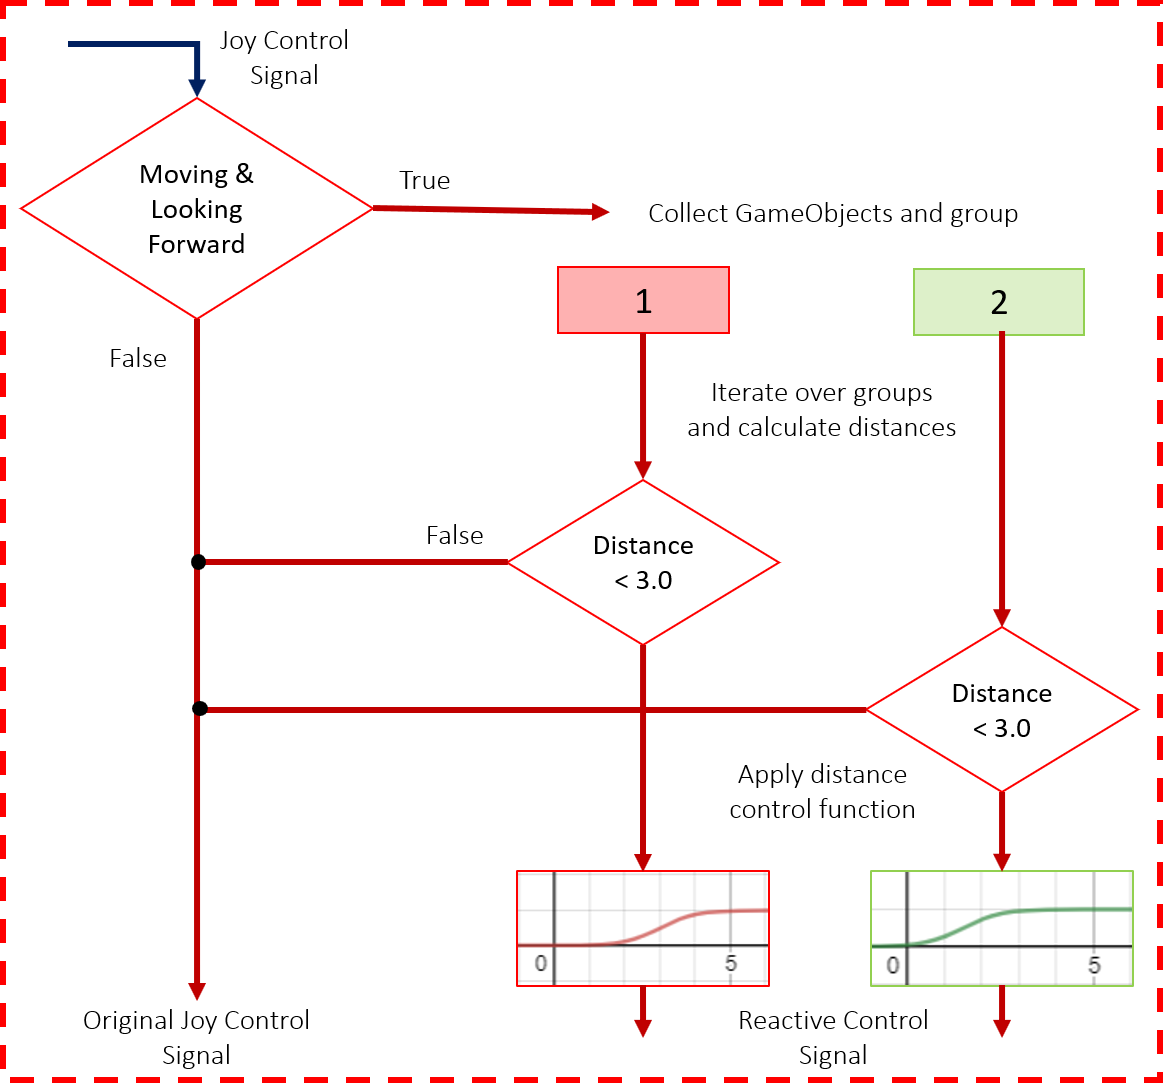
\includegraphics[width=0.8\linewidth]{img/chapter5_implementation/reactiveControlFlow.png}
    \caption{A visualization of the Reactive Control system and the corresponding distance speed scaling functions.}
    \label{fig:reactiveFlow}
\end{figure}

As aforementioned, the ideal placement of holograms for distance accuracy is between $2$ to $5$ meters. Therefore, the reactive control system checks if the detected person is less than $3$ meters away. We chose this value to give the whole system time to detect people and make a reactive decision before a collision occurs. We also check if the angle between the person and the powered wheelchair is within 15 degrees of the current trajectory. If the detection falls within both parameters, the system deems the person a collision risk, and the reactive control system takes over.

\paragraph{} Upon detecting a collision risk, the reactive control system attempts to avoid a collision by reducing the speed of the powered wheelchair. We have used two scaling functions that reduce the velocity of the wheelchair as the distance to the object decreases. If the person is directly in front of the wheelchair, the function brings the speed of the wheelchair to zero and prevents the device from moving forward until the collision risk has moved out of the way. We show these functions in Figure \ref{fig:distanceScalingFunctions}, which for people facing the wheelchair $f(x)=\frac{1}{1 + e^{-2x+6}}$ and for people walking away $f(x)=\frac{1}{1 + e^{-2x+3}}$. We chose to use different scaling since the wheelchair should slow down more quickly if a person is walking towards them.

\begin{figure}[ht]
    \centering
    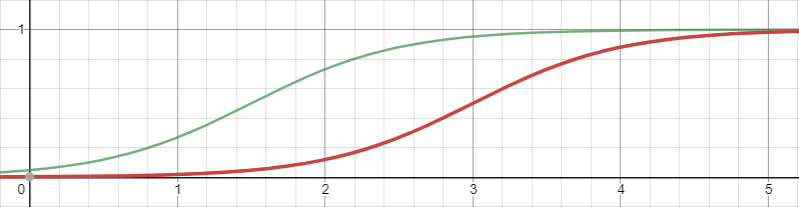
\includegraphics[width=0.8\linewidth]{img/chapter5_implementation/distanceScaling.PNG}
    \caption{The velocity scaling functions relative to the distance to the object. We note that the red function begins decreasing when the detected person is further away. This is to compensate for the person walking towards the PWU.}
    \label{fig:distanceScalingFunctions}
\end{figure} 

Finally, these modified control signals are published to ARTA. The main ARTA node receives these control signals and passes it on to the node controlling the wheels of the device.

\section{System Summary}
To summarize, we have implemented a system which utilizes the Microsoft Hololens as a form of visual input by way of the front-facing camera. The images captured by the camera are processed on an external computer. The processing begins with people detection, and the detected objects are fed into an object tracker and body pose estimation system to determine their directions. The bounding box detections and direction estimations are sent to the Hololens for spatial mapping, building a Unity scene with GameObjects that represent the detected people. Using the augmented reality capabilities of the Hololens, we render holographic visualizations for the PWU to see, indicating whether a person is walking towards them or not. Since the PWU is controlling the powered wheelchair manually, we use the reactive control system to monitor the joystick inputs from the PWU and determine whether the system should take over control from the user. If the system decides there is a collision risk in front of the powered wheelchair, it slows down the wheelchair based on the distance between the PWU and the detected person.